\documentclass[manuscript,screen]{acmart}


\IfFileExists{upquote.sty}{\usepackage{upquote}}{}
\IfFileExists{microtype.sty}{% use microtype if available
  \usepackage[]{microtype}
  \UseMicrotypeSet[protrusion]{basicmath} % disable protrusion for tt fonts
}{}
\makeatletter
\@ifundefined{KOMAClassName}{% if non-KOMA class
  \IfFileExists{parskip.sty}{%
    \usepackage{parskip}
  }{% else
    \setlength{\parindent}{0pt}
    \setlength{\parskip}{6pt plus 2pt minus 1pt}}
}{% if KOMA class
  \KOMAoptions{parskip=half}}
\makeatother

%%
%% This is file `sample-manuscript.tex',
%% generated with the docstrip utility.
%%
%% The original source files were:
%%
%% samples.dtx  (with options: `manuscript')
%% 
%% IMPORTANT NOTICE:
%% 
%% For the copyright see the source file.
%% 
%% Any modified versions of this file must be renamed
%% with new filenames distinct from sample-manuscript.tex.
%% 
%% For distribution of the original source see the terms
%% for copying and modification in the file samples.dtx.
%% 
%% This generated file may be distributed as long as the
%% original source files, as listed above, are part of the
%% same distribution. (The sources need not necessarily be
%% in the same archive or directory.)
%%
%%
%% Commands for TeXCount
%TC:macro \cite [option:text,text]
%TC:macro \citep [option:text,text]
%TC:macro \citet [option:text,text]
%TC:envir table 0 1
%TC:envir table* 0 1
%TC:envir tabular [ignore] word
%TC:envir displaymath 0 word
%TC:envir math 0 word
%TC:envir comment 0 0
%%
%%
%% The first command in your LaTeX source must be the \documentclass command.


% Options for packages loaded elsewhere
\PassOptionsToPackage{unicode}{hyperref}
\PassOptionsToPackage{hyphens}{url}
\PassOptionsToPackage{dvipsnames,svgnames,x11names}{xcolor}

\IfFileExists{bookmark.sty}{\usepackage{bookmark}}{\usepackage{hyperref}}

%% PANDOC PREAMBLE BEGINS


\providecommand{\tightlist}{%
  \setlength{\itemsep}{0pt}\setlength{\parskip}{0pt}}\usepackage{longtable,booktabs,array}
\usepackage{calc} % for calculating minipage widths
% Correct order of tables after \paragraph or \subparagraph
\usepackage{etoolbox}
\makeatletter
\patchcmd\longtable{\par}{\if@noskipsec\mbox{}\fi\par}{}{}
\makeatother
% Allow footnotes in longtable head/foot
\IfFileExists{footnotehyper.sty}{\usepackage{footnotehyper}}{\usepackage{footnote}}
\makesavenoteenv{longtable}
\usepackage{graphicx}
\makeatletter
\def\maxwidth{\ifdim\Gin@nat@width>\linewidth\linewidth\else\Gin@nat@width\fi}
\def\maxheight{\ifdim\Gin@nat@height>\textheight\textheight\else\Gin@nat@height\fi}
\makeatother
% Scale images if necessary, so that they will not overflow the page
% margins by default, and it is still possible to overwrite the defaults
% using explicit options in \includegraphics[width, height, ...]{}
\setkeys{Gin}{width=\maxwidth,height=\maxheight,keepaspectratio}
% Set default figure placement to htbp
\makeatletter
\def\fps@figure{htbp}
\makeatother

\definecolor{mypink}{RGB}{219, 48, 122}
\makeatletter
\makeatother
\makeatletter
\makeatother
\makeatletter
\@ifpackageloaded{caption}{}{\usepackage{caption}}
\AtBeginDocument{%
\ifdefined\contentsname
  \renewcommand*\contentsname{Table of contents}
\else
  \newcommand\contentsname{Table of contents}
\fi
\ifdefined\listfigurename
  \renewcommand*\listfigurename{List of Figures}
\else
  \newcommand\listfigurename{List of Figures}
\fi
\ifdefined\listtablename
  \renewcommand*\listtablename{List of Tables}
\else
  \newcommand\listtablename{List of Tables}
\fi
\ifdefined\figurename
  \renewcommand*\figurename{Figure}
\else
  \newcommand\figurename{Figure}
\fi
\ifdefined\tablename
  \renewcommand*\tablename{Table}
\else
  \newcommand\tablename{Table}
\fi
}
\@ifpackageloaded{float}{}{\usepackage{float}}
\floatstyle{ruled}
\@ifundefined{c@chapter}{\newfloat{codelisting}{h}{lop}}{\newfloat{codelisting}{h}{lop}[chapter]}
\floatname{codelisting}{Listing}
\newcommand*\listoflistings{\listof{codelisting}{List of Listings}}
\makeatother
\makeatletter
\@ifpackageloaded{caption}{}{\usepackage{caption}}
\@ifpackageloaded{subcaption}{}{\usepackage{subcaption}}
\makeatother
\makeatletter
\@ifpackageloaded{tcolorbox}{}{\usepackage[many]{tcolorbox}}
\makeatother
\makeatletter
\@ifundefined{shadecolor}{\definecolor{shadecolor}{rgb}{.97, .97, .97}}
\makeatother
\makeatletter
\makeatother
%% PANDOC PREAMBLE ENDS

\setlength{\parindent}{10pt}
\setlength{\parskip}{0pt}

\hypersetup{
  pdftitle={IS415 Report - Analysis of HDB Resale Prices},
  pdfauthor={Chen Hao Xian; Tan Wen Yang; Pierre Jean Michel},
  colorlinks=true,
  linkcolor={blue},
  filecolor={Maroon},
  citecolor={Blue},
  urlcolor={red},
  pdfcreator={LaTeX via pandoc, via quarto}}

%% \BibTeX command to typeset BibTeX logo in the docs
\AtBeginDocument{%
  \providecommand\BibTeX{{%
    Bib\TeX}}}

%% Rights management information.  This information is sent to you
%% when you complete the rights form.  These commands have SAMPLE
%% values in them; it is your responsibility as an author to replace
%% the commands and values with those provided to you when you
%% complete the rights form.
\setcopyright{acmcopyright}
\copyrightyear{2023}
\acmYear{}
\acmDOI{}

%% These commands are for a PROCEEDINGS abstract or paper.
\acmConference[]{}{}{}
\acmPrice{}
\acmISBN{}

%% Submission ID.
%% Use this when submitting an article to a sponsored event. You'll
%% receive a unique submission ID from the organizers
%% of the event, and this ID should be used as the parameter to this command.
%%\acmSubmissionID{123-A56-BU3}

%%
%% For managing citations, it is recommended to use bibliography
%% files in BibTeX format.
%%
%% You can then either use BibTeX with the ACM-Reference-Format style,
%% or BibLaTeX with the acmnumeric or acmauthoryear sytles, that include
%% support for advanced citation of software artefact from the
%% biblatex-software package, also separately available on CTAN.
%%
%% Look at the sample-*-biblatex.tex files for templates showcasing
%% the biblatex styles.
%%

%%
%% The majority of ACM publications use numbered citations and
%% references.  The command \citestyle{authoryear} switches to the
%% "author year" style.
%%
%% If you are preparing content for an event
%% sponsored by ACM SIGGRAPH, you must use the "author year" style of
%% citations and references.
%% Uncommenting
%% the next command will enable that style.
%%\citestyle{acmauthoryear}


%% end of the preamble, start of the body of the document source.
\begin{document}


%%
%% The "title" command has an optional parameter,
%% allowing the author to define a "short title" to be used in page headers.
\title{IS415 Report - Analysis of HDB Resale Prices}

%%
%% The "author" command and its associated commands are used to define
%% the authors and their affiliations.
%% Of note is the shared affiliation of the first two authors, and the
%% "authornote" and "authornotemark" commands
%% used to denote shared contribution to the research.


  \author{Chen Hao Xian}
  
    \author{Tan Wen Yang}
  
    \author{Pierre Jean Michel}
  
            \affiliation{%
                  \institution{Singapore Management University}
                                  \city{Singapore}
                                  \country{Singapore}
                      }
      

%% By default, the full list of authors will be used in the page
%% headers. Often, this list is too long, and will overlap
%% other information printed in the page headers. This command allows
%% the author to define a more concise list
%% of authors' names for this purpose.
%\renewcommand{\shortauthors}{Trovato et al.}
%%  
%% The abstract is a short summary of the work to be presented in the
%% article.
\begin{abstract}
\textbf{Abstract} This research aims to provide Singaporeans with a
better understanding of the factors impacting the resale price of HDB
flats, given the lack of accessible geographically weighted models. The
study uses geographically weighted regression models to identify the
most significant location-specific variables affecting resale prices,
such as proximity to rail stations, hawker centers, preschools, mall,
and etc. Furthermore, a user-friendly web application has been developed
to estimate the resale value of HDB flats based on these variables. This
tool will help homeowners, buyers, and policymakers make more informed
decisions about the HDB resale market and ultimately lead to better
outcomes.    
\end{abstract}

%%
%% The code below is generated by the tool at http://dl.acm.org/ccs.cfm.
%% Please copy and paste the code instead of the example below.
%%

%%
%% Keywords. The author(s) should pick words that accurately describe
%% the work being presented. Separate the keywords with commas.
\keywords{HDB Prices, Linear Regression, Geographically Weighted
Regression, Exploratory Data Analysis}


%%
%% This command processes the author and affiliation and title
%% information and builds the first part of the formatted document.
\maketitle

\setlength{\parskip}{-0.1pt}

\hypertarget{motivation}{%
\section{Motivation}\label{motivation}}

With the price of HDB resale flats seeing tremendous growth over the
years, and news such as ``\textbf{HDB resale prices accelerate in Jan as
million-dollar deals surge by 42\%: SRX, 99.co''} \citep{Yong23} or
\textbf{``HDB resale prices rise 2.3\% in Q4, slowest increase in
2022''} \citep{Liew23}, Singaporeans face the ever-growing concern as to
whether or not they are paying a fair price for their flats. Given the
lack of accessibility to geographically weighted models, users may find
it difficult to assess what factors impact the resale price of an HDB
flat; indeed, current estimators often only consider linear
relationships between dependent and independent variables and fail to
include geographical predictors in their models, which may limit the
ability of one regression to explain HDB resale prices; however,
geographically weighted regressions provide a more sophisticated way to
model spatial heterogeneity by accounting for the unique characteristics
of different neighborhoods.

Despite the advantages of geographically weighted regressions, they can
be difficult for casual users without specialized skills to use
effectively. Thus, our research comes in handy to give the right tools
to Singaporeans as we aim to:

\begin{enumerate}
\def\labelenumi{\arabic{enumi}.}
\item
  Identify the most significant location-specific variables that affect
  the resale price of HDB flats in Singapore and quantify their impact
  on pricing using geographically weighted regression models. By
  analyzing the relationship between different amenities, such as rail
  stations, hawker centers, preschools, malls, and more. We aim to
  determine which factors have the most significant explanatory power on
  HDB resale prices and which do not. It will provide valuable insights
  into the most important factors that home buyers and sellers should
  consider when transacting in the HDB resale market.
\item
  Develop a user-friendly web application that leverages geographically
  weighted regression models to estimate the resale value of HDB flats
  in Singapore for a given area. By inputting location-specific
  variables such as proximity to rail stations, hawker centers,
  preschools, malls, and etc. users can receive an estimated resale
  value for their property. It will provide users with a more accurate
  estimation of the value of their property, which can help them make
  better decisions when selling or buying an HDB flat.
\item
  Promote transparency and reduce information asymmetry in the HDB
  resale market by providing an accessible and user-friendly tool for
  estimating resale values. By making geographically weighted regression
  models more accessible to the public, we hope to empower homeowners,
  buyers, and policymakers to make more informed decisions about the HDB
  resale market. It could ultimately lead to better outcomes for buyers
  and sellers and help policymakers make more informed decisions about
  housing affordability, urban planning, and education policy.
\end{enumerate}

\hypertarget{relevant-related-work}{%
\section{Relevant Related Work}\label{relevant-related-work}}

We will now discuss past research in the fields of hedonic housing price
models and the importance of geography in these models. We shall review
three pieces of work in the following paragraphs.

Our first article \citep{helbich2013}, ``Spatial Heterogeneity in
Hedonic House Price Models: The Case of Austria.'' by M. Helbich, C.
Leitner, and A. Kapusta, investigates the spatial heterogeneity of
housing prices in Austria by using a hedonic pricing model. This
statistical model estimates the value of a property based on its
attributes, size, location, and other factors, such as proximity to
different amenities (e.g., shopping malls and parks). In this paper, the
writers apply geographically weighted regression (GWR) analysis to
identify local spatial patterns of the housing market and examine the
spatial variability of the hedonic price model coefficients. In their
research, they deduce that the GWR approach provides more accurate
predictions of housing prices than traditional regression methods, which
assume spatial homogeneity of coefficients. Their study revealed that
housing prices are significantly influenced by local characteristics of
neighborhoods as accessibility, environment, and social amenities, to
name a few. Their paper suggests that the spatial heterogeneity of
housing prices is crucial to accurately model and analyze the housing
market, especially in geographically diverse regions like Austria. In
our case, we consider the paper's methodology and insights valuable for
our research as we plan to investigate the spatial heterogeneity of
housing prices in Singapore and identify local factors that affect house
prices.

The second work we will analyze is the
\href{https://services2.hdb.gov.sg/webapp/BB33RTIS/}{HDB Resale Flat
Prices} \citep{HDBapp} application developed by the Housing Development
Board of Singapore. It provides a platform for users to access
information on past resale transactions of Housing and Development Board
(HDB) flats in Singapore. It allows users to search for resale
transactions based on various criteria, such as location, flat type, and
transaction period. This web application is the perfect example of what
Singaporeans are missing, a model that explains the relevancy of
locational factors on HDB resale price. Nonetheless, this web
application still serves as a relevant solution that offers insights
into the Singapore housing market and the attributes of HDB flats that
may affect transaction prices. We believe there is room for improvement
in the functionalities the platform offers. Through our research, we aim
to explore ways to improve the current system, perhaps by incorporating
additional data sources and applying advanced machine learning
algorithms to provide an accurate and valuable explanatory model of
housing prices.

The last piece of reading we shall discuss is the Medium article
\citep{Kok21} ``Predict the Selling Price of HDB Resale Flats'' by Jim
Meng Kok. It uses machine learning to predict the selling price of HDB
resale flats in Singapore. The author uses a dataset of HDB resale
transactions and applies a random forest regression model to predict the
resale price of HDB flats based on various features, including location,
size, age, and nearby amenities. The model achieves a high accuracy
rate, indicating that machine learning methods can effectively predict
housing prices. The article is relevant to the current research on
housing prices in Singapore as it highlights the importance of utilizing
machine learning techniques for predicting prices accurately. While the
author uses Python in his analysis, we still consider that the insights
provided in the article can be valuable for any researcher planning to
use other programming languages, as R. The findings suggest that
location and amenities play a significant role in determining housing
prices, which is consistent with previous research on the topic.

In conclusion, this section has reviewed three pieces of research
related to hedonic housing price models and the importance of geography
in these models. Overall, these studies emphasize the need to account
for location and amenities when modeling and analyzing housing prices
and highlight the potential of advanced techniques like geographically
weighted regression and machine learning to provide more accurate
predictions.\\

\hypertarget{design-framework}{%
\section{\texorpdfstring{\textbf{Design
Framework}}{Design Framework}}\label{design-framework}}

The design of our Shiny App tries to follow the data visualization
general guidelines suggested by Schneiderman's mantra
\citep{shneiderman}: Overview First, Zoom and Filter, Details on Demand.
It consists of Eight Different Tabs: About Us, EDA, CorrPlot, Multiple
Linear Regression, Geographically Weighted Regression, Predicting,
Interactive Map and Upload File {[}Figure 1{]} Figure~\ref{fig-1}. This
Navigation Bar is featured throughout all the Shiny App at all time.
Each of the Features are place in the order where the user is expected
to navigate in. Each of the Tab Features is own unique set of features,
however there are 3 major views, map, graphic and tables.

About Us Tab (Figure~\ref{fig-1}) is an overview of application and
features no interactivity.

The EDA Tab (Figure~\ref{fig-2}) features an overview of the entire data
set that is loaded in the Shiny Model. A Histogram is given to give an
overview of selected variable of the data set. Key Summaries is also
provide important information that the user might need, such as the
summary of the data and the Top 10 towns. This information is given in a
form of a table. Finally, the entire data is given in the form of the
table for the user to view the entire data. The Shiny Application
provide a sidebar, where all the drop downs form are located. We namely
allow the user to modify the Start Date, End Date and the Room Type. For
the Histogram, the user is able to select the number of bins, the color
of the Fill and the data to be displayed.

The Corr Plot Tab (Figure~\ref{fig-3}) features a Graphic Plot of
Correlation Plot of the variables. The Correlation Plot is calculated
based on the columns of the data set.

The Multiple Linear Regression Tab (Figure~\ref{fig-4}) features
graphics of the Linear Regression Model. It also features all the
various test to determine the validity of the Linear Regression Model,
such as Linearity and Moran I for the Spatial Model. All the outputs are
featured as a graphic with explanation on what to look out for. The Side
Bar Features a multi select drop down of all the dependent variables of
the data set to build the Linear Regression Model. Changing the values
in the Multi Select will update all the graphics with the exception of
Moran I as it is computationally intensive. As weight matrix is needed
to calculate Moran I, as many variables of dnearneight() and nb2listw()
function is exposed \citep{spdep}.

The Geographically Weighted Regression Tab (Figure~\ref{fig-5}) features
graphics of the Geographically Weighted Regression and the explanation
needed. The current graphics of the GWR Model is not computed
re-actively as the the computation of the bandwidth and the model is
computationally intensive. The side bar features as many variables of
bw.gwr() and gwr.basic() function is exposed \citep{GWmodel}. Two
buttons named `Generate GWR' and `Use Computed BandWidth' can be used to
render the graphic re-actively but it will take a long time to load.

The Predict Tab (Figure~\ref{fig-6}) features a simple graphic of the
predict values. The side bar provides the ability to toggle between the
GWR Model or the Linear Regression Model. The GWR Model requires a
Spatial Model to be uploaded, while the Regression Model requires input
on a text box, separated by comma.

The Interactive Map Tab (Figure~\ref{fig-7}) features an interactive Map
of all the Points in the data set. The user can filter out the Start
Date, End Date and Room Type of the data set to display. Any columns in
the data set can be displayed on the interactive map and some options of
the well know colorbrewer \citep{colorbrewer} is given for the user to
select. The user can select the classification methods of the points
from a drop down, based on attributes available from tmap package
\citep{tmap}. The tab is place towards the end because the interactive
map is not the main objective of this project but provided the user to
gain a better understanding of the data.

The Upload File Tab (Figure~\ref{fig-8}) features a Table that is only
displayed when the user upload a file. The user can upload a file from
the sidebar. This tab is placed at the end, as the user should gain a
better understanding of the ability of our application attempting to
load their own data.

A combination of these three views along with the ability to build their
own model based on their own judgement should give the user a great
control over the data and more power to analyze and explore.

\hypertarget{case-study-of-hdb-resale-flats}{%
\section{\texorpdfstring{\textbf{Case Study of HDB Resale
Flats}}{Case Study of HDB Resale Flats}}\label{case-study-of-hdb-resale-flats}}

Singapore, an emerging economy with a thriving real estate market,
boasts a unique housing landscape that has drawn attention worldwide.
Indeed, Singapore is one of the few city-states in the world, making it
a compact and densely populated urban environment. This unique
characteristic could already be the foundation of a fascinating use case
for our web app. Yet, what makes Singapore housing so special is the
government's active role in shaping the market, which has led to the
development of the Housing and Development Board (HDB) flats -- an
essential feature of the Singaporean housing landscape.~

Since the 1960s, the Singaporean government has heavily involved itself
in public housing, and its policies have gained widespread recognition
for their success. The country's housing policies have been instrumental
in promoting homeownership and providing affordable housing for its
citizens. These flats, built and managed by the government, house over
80\% of the population \citep{Harsh22}, making Singapore's public
housing program one of the most successful in the world. The HDB flats,
however, are subject to unique rules and regulations that distinguish
them from other housing solutions (e.g., private housing), such as
restrictions on resale and renovation. Thus, understanding the factors
that drive the prices of HDB resale flats is of great interest. In this
context, geographically weighted regression analysis is an ideal method
for examining the spatial heterogeneity of HDB resale prices and
identifying the local factors that influence them. By considering the
specific characteristics of each HDB estate and the surrounding
neighborhoods, we can better understand how various factors, such as
distance to amenities, transport links, and schools, affect the prices
of HDB resale flats. With our web app, policymakers, investors, and
residents can use these insights to make more informed decisions about
the HDB market.

To analyze the spatial heterogeneity of HDB prices in Singapore, we will
utilize a variety of variables that capture different aspects of the
flats and their surrounding areas. These variables include AREA\_SQM,
LEASE\_YRS, STOREY\_ORDER, and proximity to various amenities such as
CBD, childcare, eldercare, hawker centers, MRT stations, parks, top
primary schools, malls, supermarkets, clinics, pharmacies, tourist
attractions, and libraries. We have sourced this data from websites such
as data.gov.sg, Wikipedia, LTA Data Mall, and the MOE website, and
additionally used the OneMap API to retrieve and geocode data. Some data
preprocessing was necessary as geocoding aspatial fields to convert
addresses into geographic coordinates. Using geographically weighted
regression analysis on this rich dataset, we can identify local factors
that influence the prices of HDB resale flats in different regions of
Singapore.~

For the sake of limiting the computing power required to run our
analysis, we shall only focus on HDB resale flat transactions from 2021
to 2022. This can be done at the EDA Tab, where the user will filter out
the data into the correct time frame. It would appears that the PRICE
variable is left-skewed base on the Histogram. Altering the display
variable to LEASE\_YRS will give a different picture, where the data is
right-skewed. Key Summaries of the variable such as the median and mean
will be displayed. The mean of the variable based on towns will be
displayed as well. From the PRICE variable, the mean is found to be
526124 and the Central Area has the highest mean PRICE.

The Multiple Linear Regression (MLR) model reveals that most variables
have a statistically significant effect on housing prices in Singapore
(Figure~\ref{fig-9}). The intercept is estimated to be 1.607e+05,
indicating that a house with all predictor variables set to zero should
cost at least \textbf{S\$160,700}. The variables that positively impact
housing prices are AREA\_SQM, LEASE\_YRS, STOREY\_ORDER, PROX\_PARK,
NUM\_KNDRGTN, NUM\_ISP\_CLIN, and NUM\_REGISTERED\_PHARM, while the
variables with a negative impact are PROX\_CBD, PROX\_HAWKER, PROX\_MRT,
PROX\_MALL, PROX\_SPRMKT, PROX\_PHARMACY, and PROX\_TOURISM. The
variable PROX\_CLINIC has a p-value of 0.47737 and is not statistically
significant at a 5\% error level. Meanwhile AGE and PROX\_TOPPRISCH
since to return a null result. The R-squared value of 0.7381 indicates
that the model's predictor variables can explain 73.81\% of the variance
in housing prices. The F-statistic of 3171 with a p-value of \textless{}
2.2e-16 suggests that the model's overall fit is significant.

We must however understand that Linear Regression Model has a number of
key assumptions namely: \emph{Linearity, Normality, Homoscedasticity and
Independence} \citep{ernst2017}\emph{.} We have conducted all of this
test and have determine that our model satisfy this criteria.

Independence Test is already performed at in the Corr Plot Tab
(Figure~\ref{fig-3}). All variables that are correlated should be remove
already. We have kept all the variables in our default model for
demonstration purposes however.

Linearity Test (Figure~\ref{fig-10}) performed have shown that
LEASE\_YRS, AGE, PROX\_MRT and PROX\_TOPPRISCH have a VIF more than 10

Homoscedasticity Test (Figure~\ref{fig-11}) performed have shown that
most of the residual is scattered around the line, however there are
points that deviate significantly from the line.

Normality Test (Figure~\ref{fig-12}) performed have shown that most of
the residual resembles a Normal Distribution Curve.

Furthermore, in this study, we conducted a global Moran's I test to
assess the presence of spatial autocorrelation in housing prices in
Singapore. Our results showed a Moran I statistic standard deviate of
1122.3 and a p-value smaller than 2.2e-16 (Figure~\ref{fig-13}),
indicating strong evidence of spatial autocorrelation in resale HDB
flats. Specifically, our observed Moran I was 0.217. It is significantly
higher than the expected value under spatial randomness. It demonstrates
the significance of spatial autocorrelation in housing prices in
Singapore, and we should consider it for several reasons.

First, it suggests that housing prices in some regions of the city-state
are not independent and that the prices of nearby properties may
influence resale value. It means that traditional regression techniques,
which assume independence between observations, may need to be revised
for modeling housing prices in Singapore.

Moreover, spatial autocorrelation can reveal the underlying spatial
structure of housing prices in Singapore, including spatial patterns and
trends. Understanding these patterns can provide valuable insights into
the factors that drive housing prices in different parts of the country.
Empirical evidence also supports the relevance of spatial
autocorrelation in housing prices. For example, a study by Wong and
Leung \citep{chunwah2011} found significant spatial autocorrelation in
housing prices in Hong Kong and suggested that spatial models, such as
geographically weighted regression, could improve the accuracy of price
predictions.

While the MLR model provides valuable insights into the relationship
between the predictor variables and housing prices, it does not consider
the spatial variation in the data. Therefore, it may need to capture the
heterogeneity observed in different regions of Singapore fully. To
address this issue, we will employ a geographically weighted regression
(GWR) model, allowing us to examine how the relationship between the
predictor variables and housing prices varies spatially across different
regions of Singapore.

A GWR Model is build using the exact same data set which result in a
R-Squared value of -22174.95 (Figure~\ref{fig-14}). This is likely due
to the fact that the model used was not fine tuned at all. When the same
data set is used by Megan and Aisyah, such model produced a R-squared
value of 0.9 and greater \citep{sim23} \citep{Aisyah}. This shows that
the model has the potential to be significantly better than the
Regression Model when proper tuning is performed.

This case study have shown that with the available data, the user is
able to gain insights on the data through the EDA. The user is able to
make use of the interactive nature of the Shiny Application to focus on
a specific variable of interest and make a judgement on whether the
variable should be included in the model. The user can reference the
CorrPlot and the various Linear Model Tests to gain insights of the
relationship between the variables to choose the variables used in the
Linear Regression Model and Geographically Weighted Model. This will
definitely encourage the user to explore the data and fine tune the
Model for more in depth exploration and Analysis.

\hypertarget{conclusion}{%
\section{\texorpdfstring{\textbf{Conclusion}}{Conclusion}}\label{conclusion}}

We have used geographically weighted regression models to explore the
spatial variation of HDB resale prices in Singapore and to identify the
location-specific factors that influence them. We have found that the
distance to various amenities, such as rail stations, hawker centers,
preschools, malls, and more, have different effects on HDB resale prices
depending on the location and that some factors are more relevant than
others in accounting for the spatial heterogeneity of resale prices. We
have also created interactive maps to visualize the spatial patterns of
these factors and their impacts on pricing. Moreover, we have developed
a user-friendly web application that uses geographically weighted
regression models to allow users to estimate the fair value of any HDB
flat based on its location and features. Our web application can assist
users in making informed choices when buying or selling HDB flats in the
resale market and also enhance their understanding of the spatial
dynamics of HDB resale prices in Singapore.

\hypertarget{potential-future-work}{%
\section{\texorpdfstring{\textbf{Potential Future
Work}}{Potential Future Work}}\label{potential-future-work}}

Our Model can be expanded in number of key areas as the potential for
the application to grow is large.

We can expand the scope of the project to encompass the Private
Properties and the introduction of new geographical variable as well.
The addition of Private Properties prices will give a more complete view
of the housing situation in Singapore, which can result in a much better
model. The addition of geographical data as well can also be critical as
geographical data of interesting variables such as Hospital, Tourist
Attraction has not be included in the loaded model. The inclusion of
such geographical data into the data set can give more insights to the
user as it may review surprising relationship.

We can also expand the number of models that the project uses as well.
In this project only Linear Regression Model and Geographically Weighted
Regression is used. Models such as Geographically Weighted Regression
Trees can be introduced for the user to further compare and contrast.
Some of these possible enhancements could be taken up in the near
future.

\hypertarget{appendices}{%
\section{Appendices}\label{appendices}}

\hypertarget{bibliography}{%
\subsection{Bibliography}\label{bibliography}}

\bibliographystyle{ACM-Reference-Format}

\bibliography{bibliography.bib}

\hypertarget{figures}{%
\subsection{Figures}\label{figures}}

\begin{figure}

{\centering 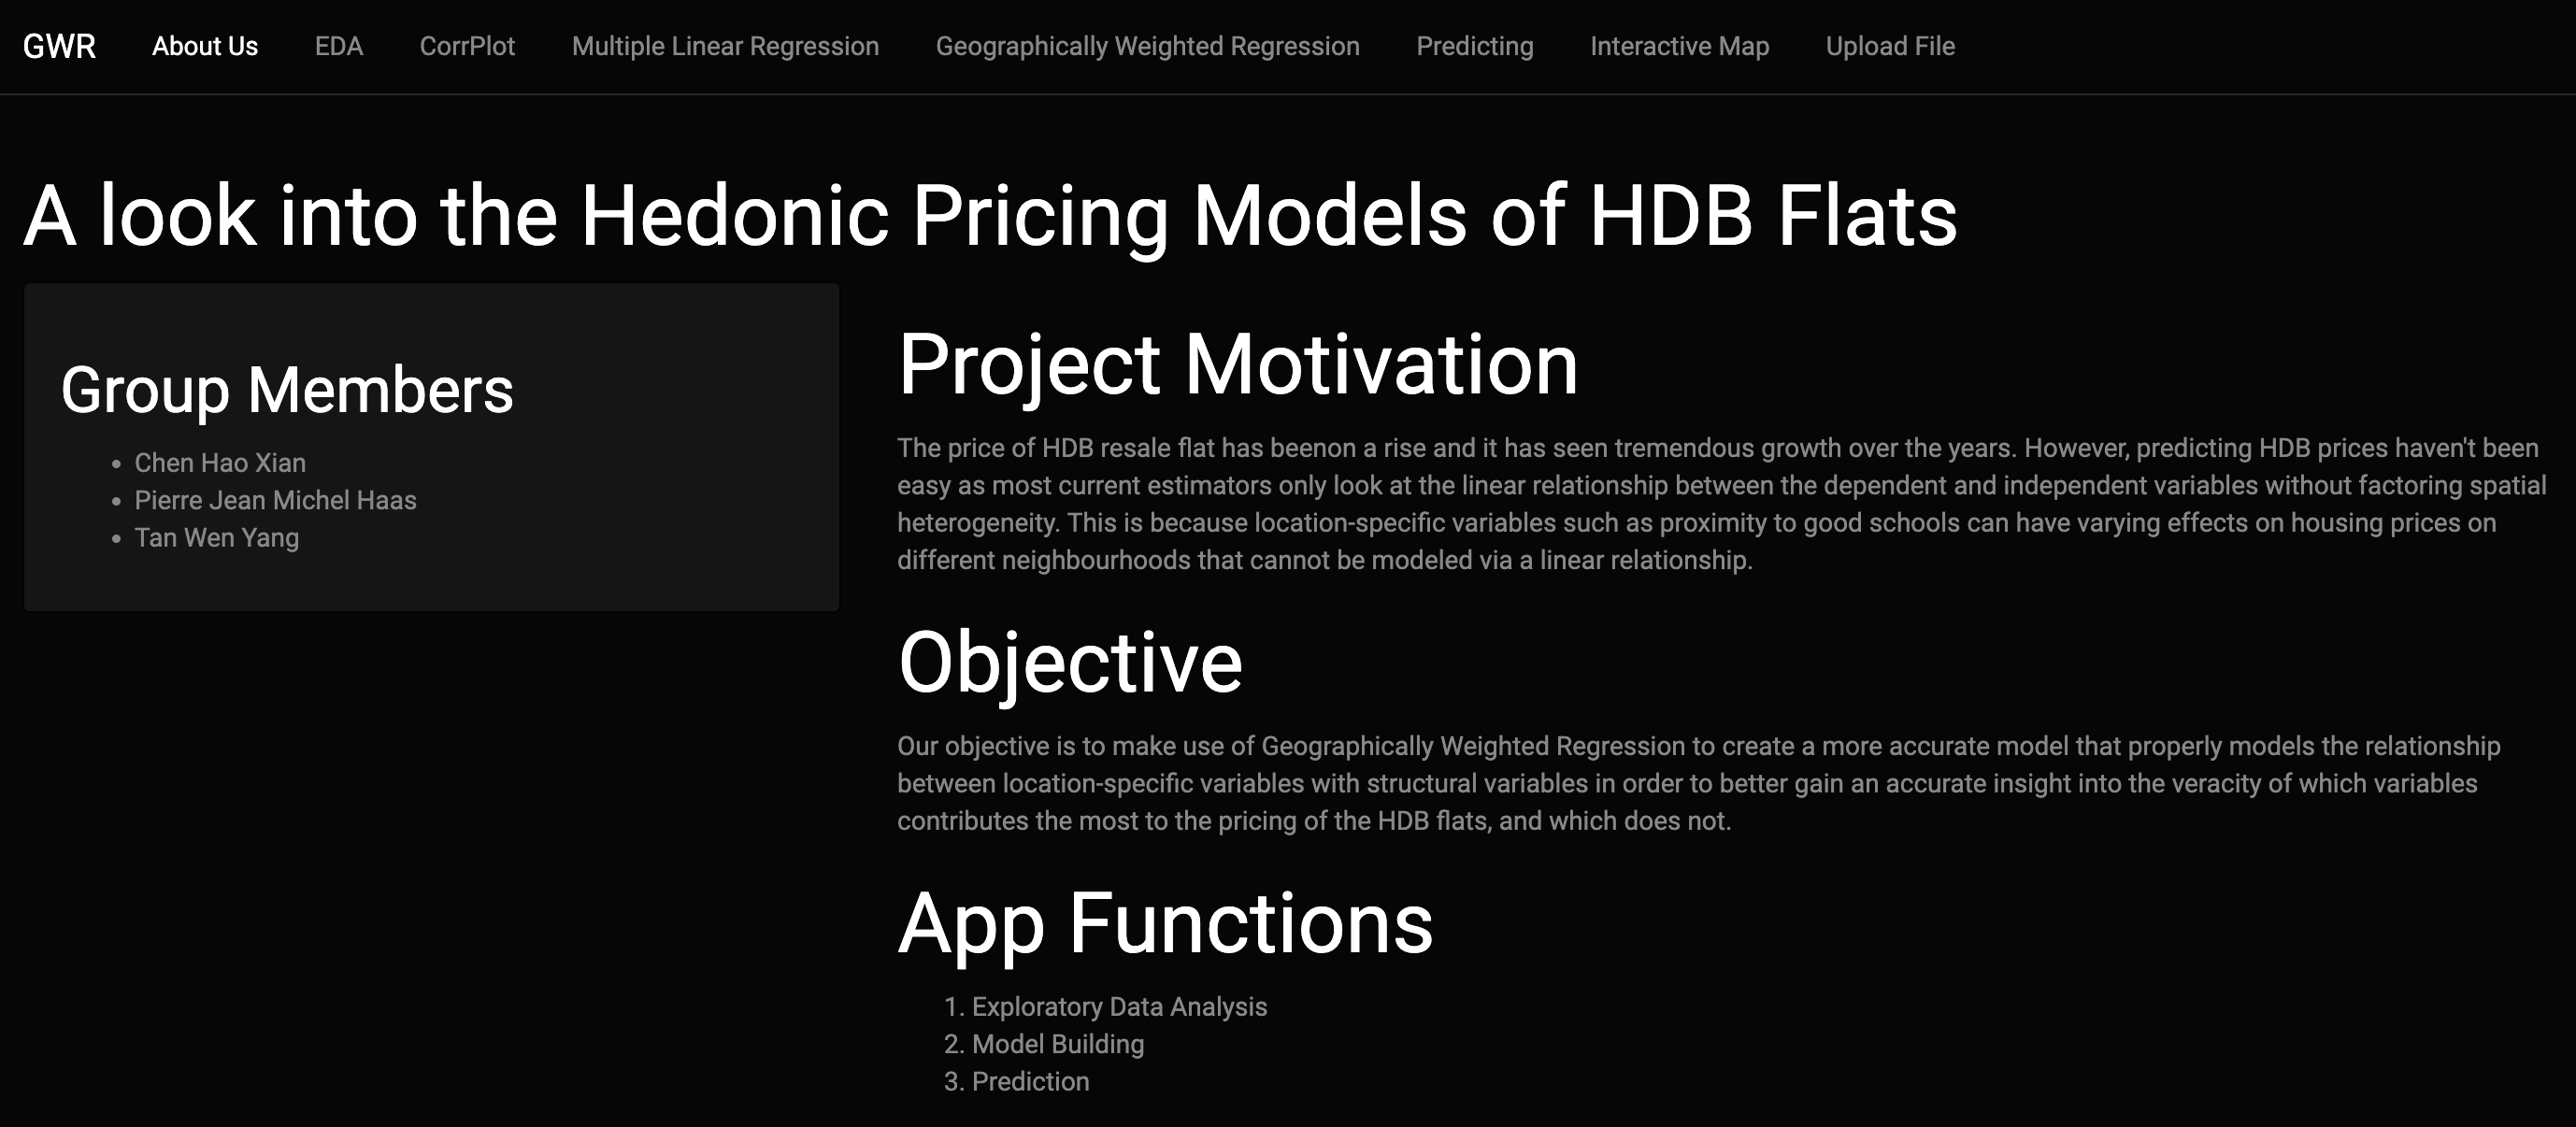
\includegraphics{images/Screenshot 2023-04-14 at 11.08.12 PM.png}

}

\caption{\label{fig-1}About Us Tab}

\end{figure}

\begin{figure}

{\centering 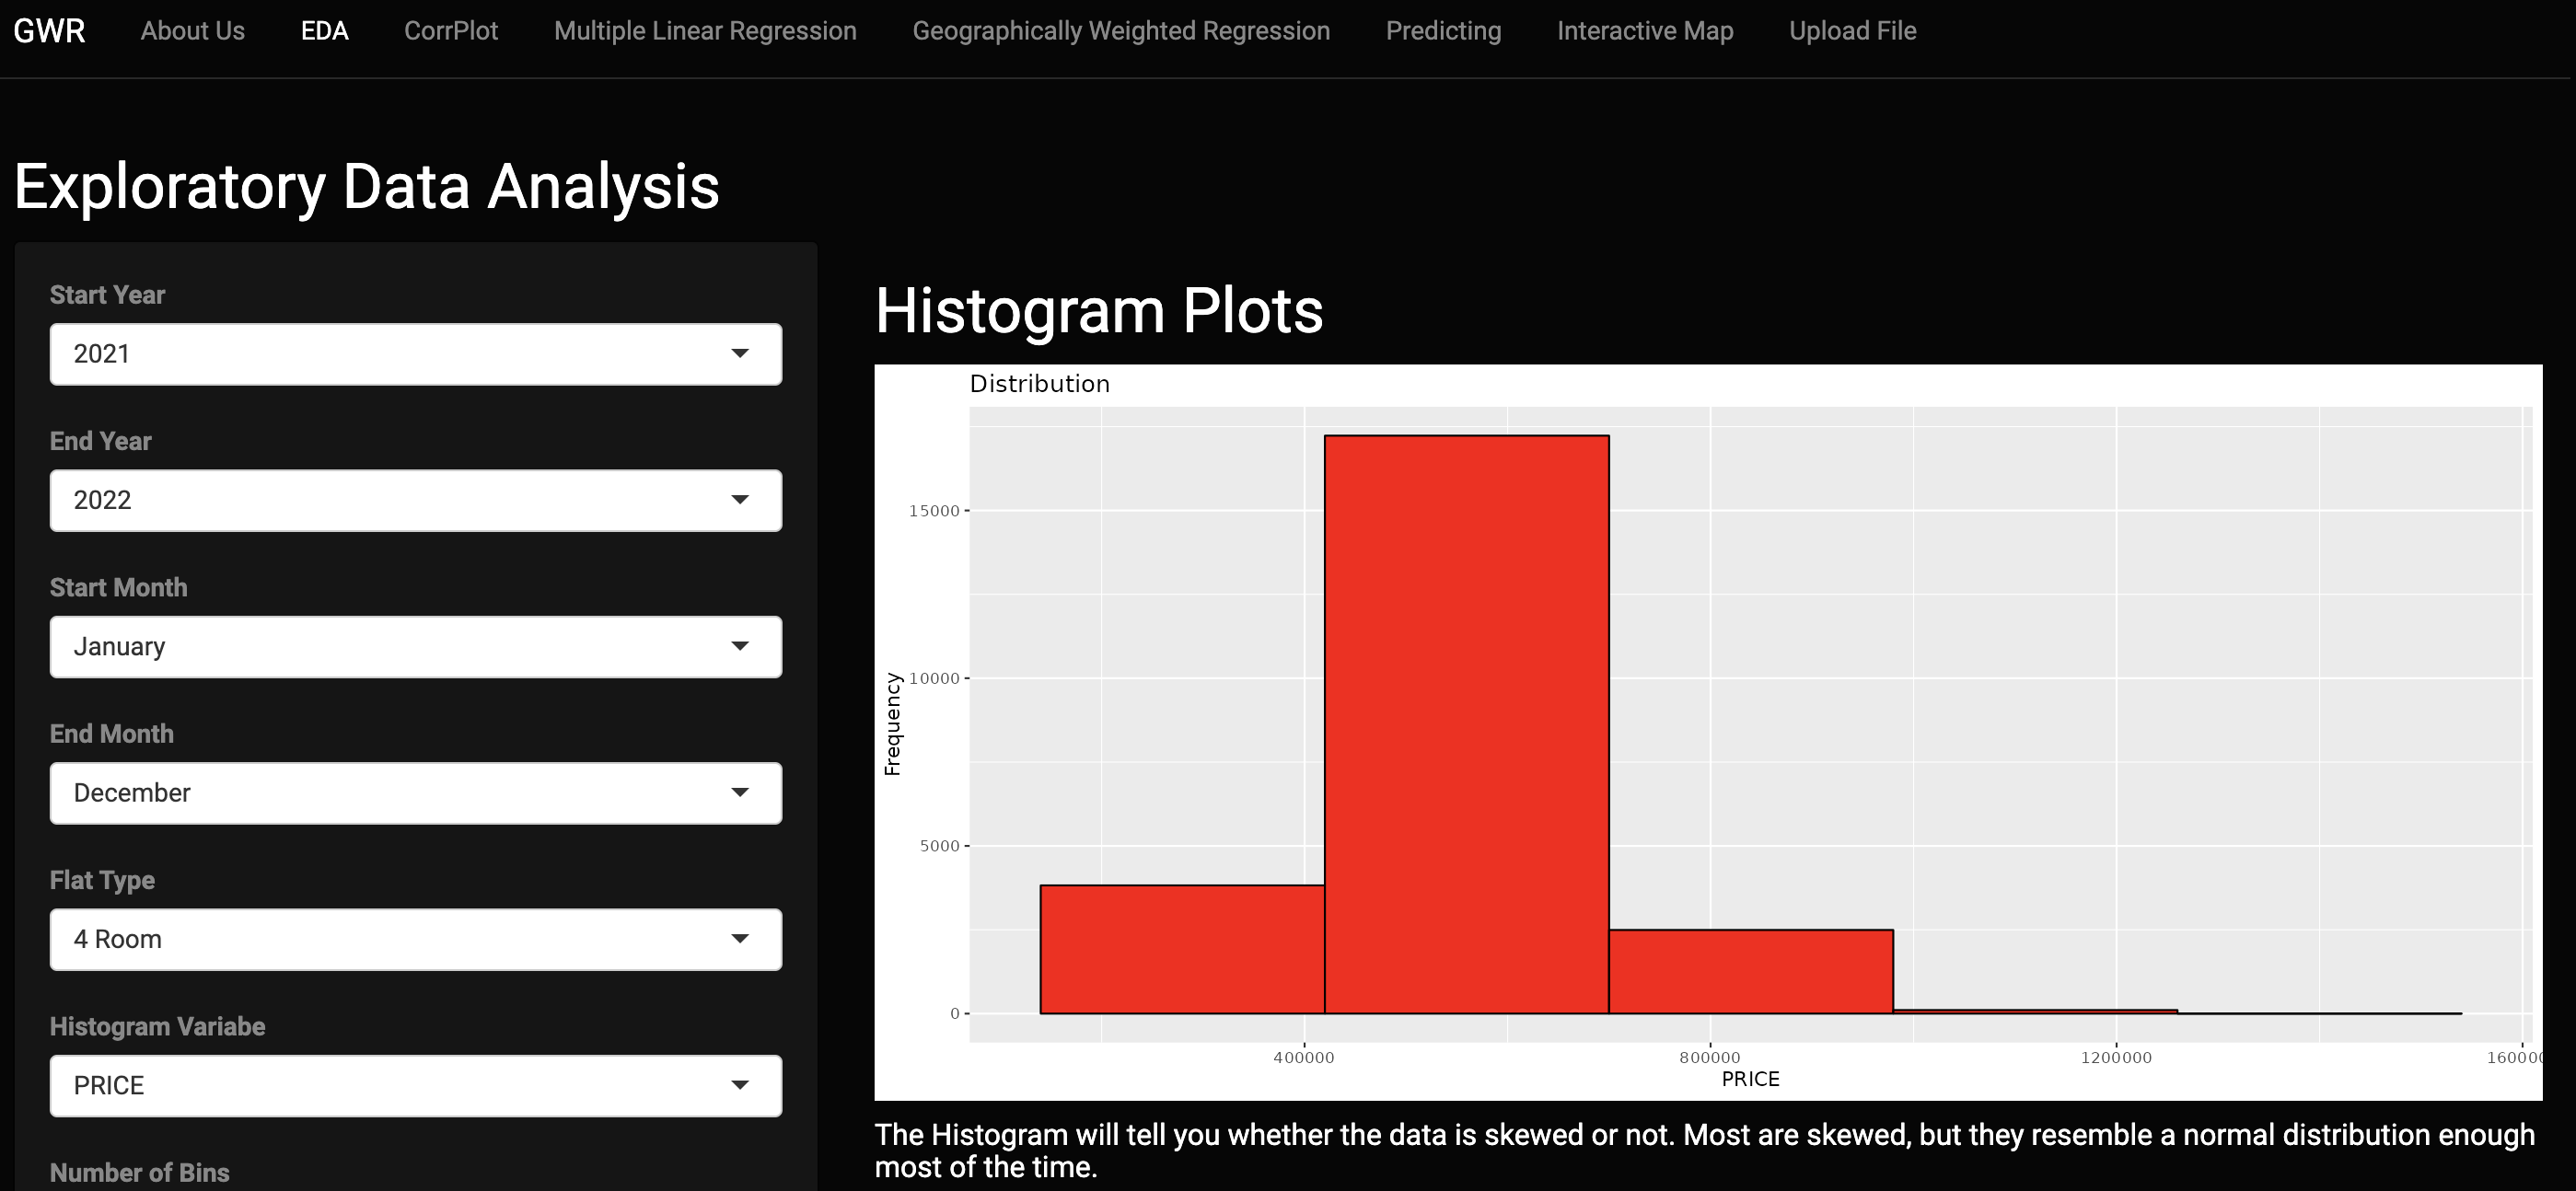
\includegraphics{images/Screenshot 2023-04-14 at 11.34.06 PM.png}

}

\caption{\label{fig-2}EDA Tab}

\end{figure}

\begin{figure}

{\centering 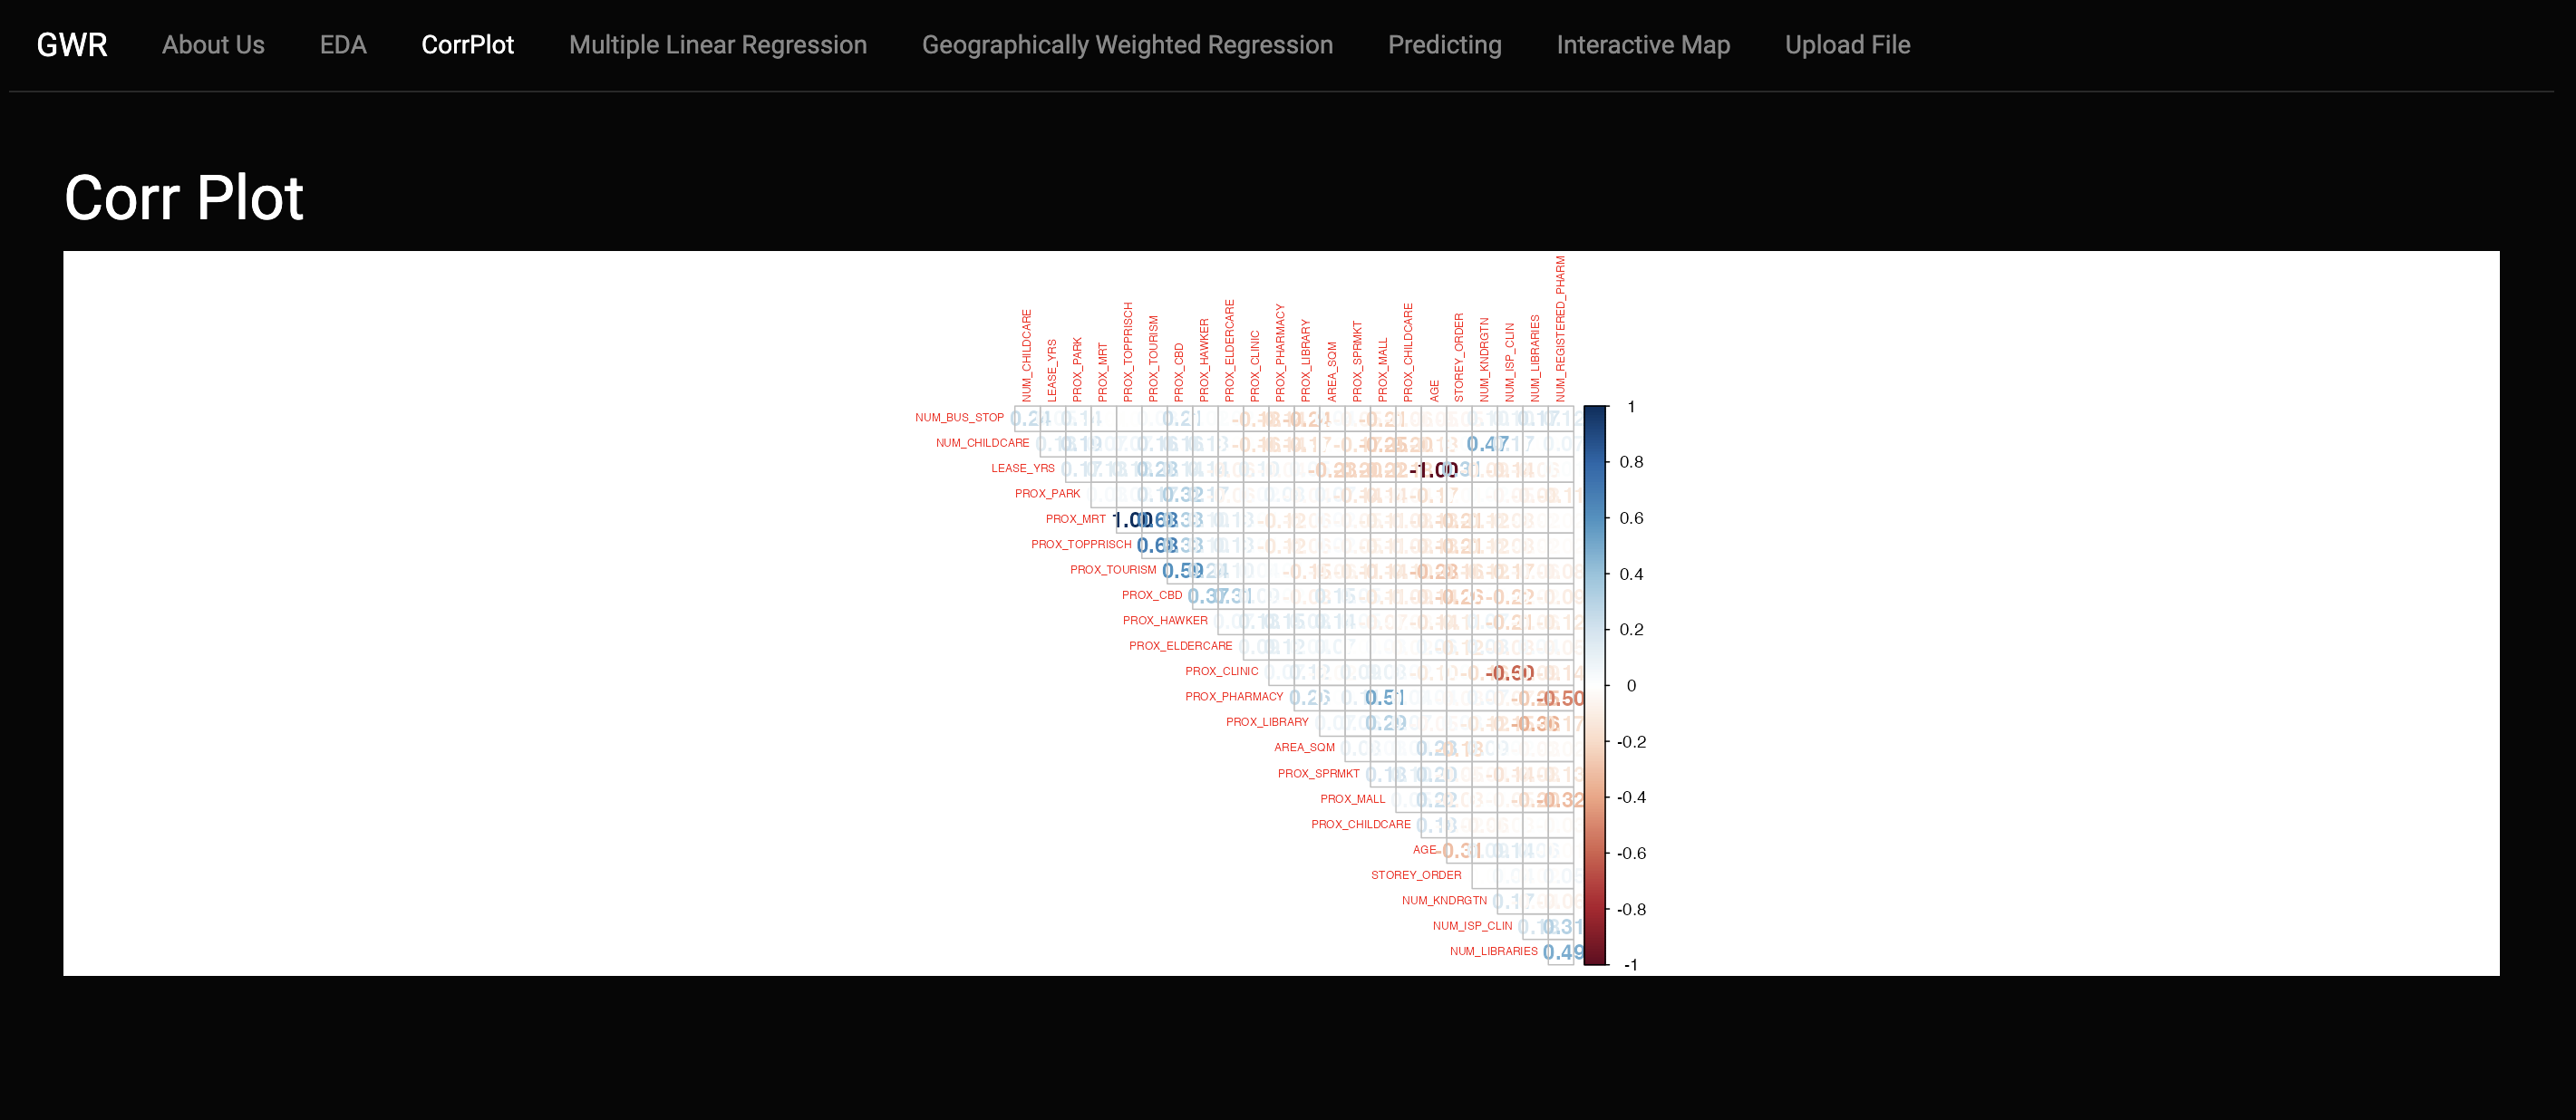
\includegraphics{images/Screenshot 2023-04-14 at 11.41.50 PM.png}

}

\caption{\label{fig-3}CorrPlot Tab}

\end{figure}

\begin{figure}

{\centering 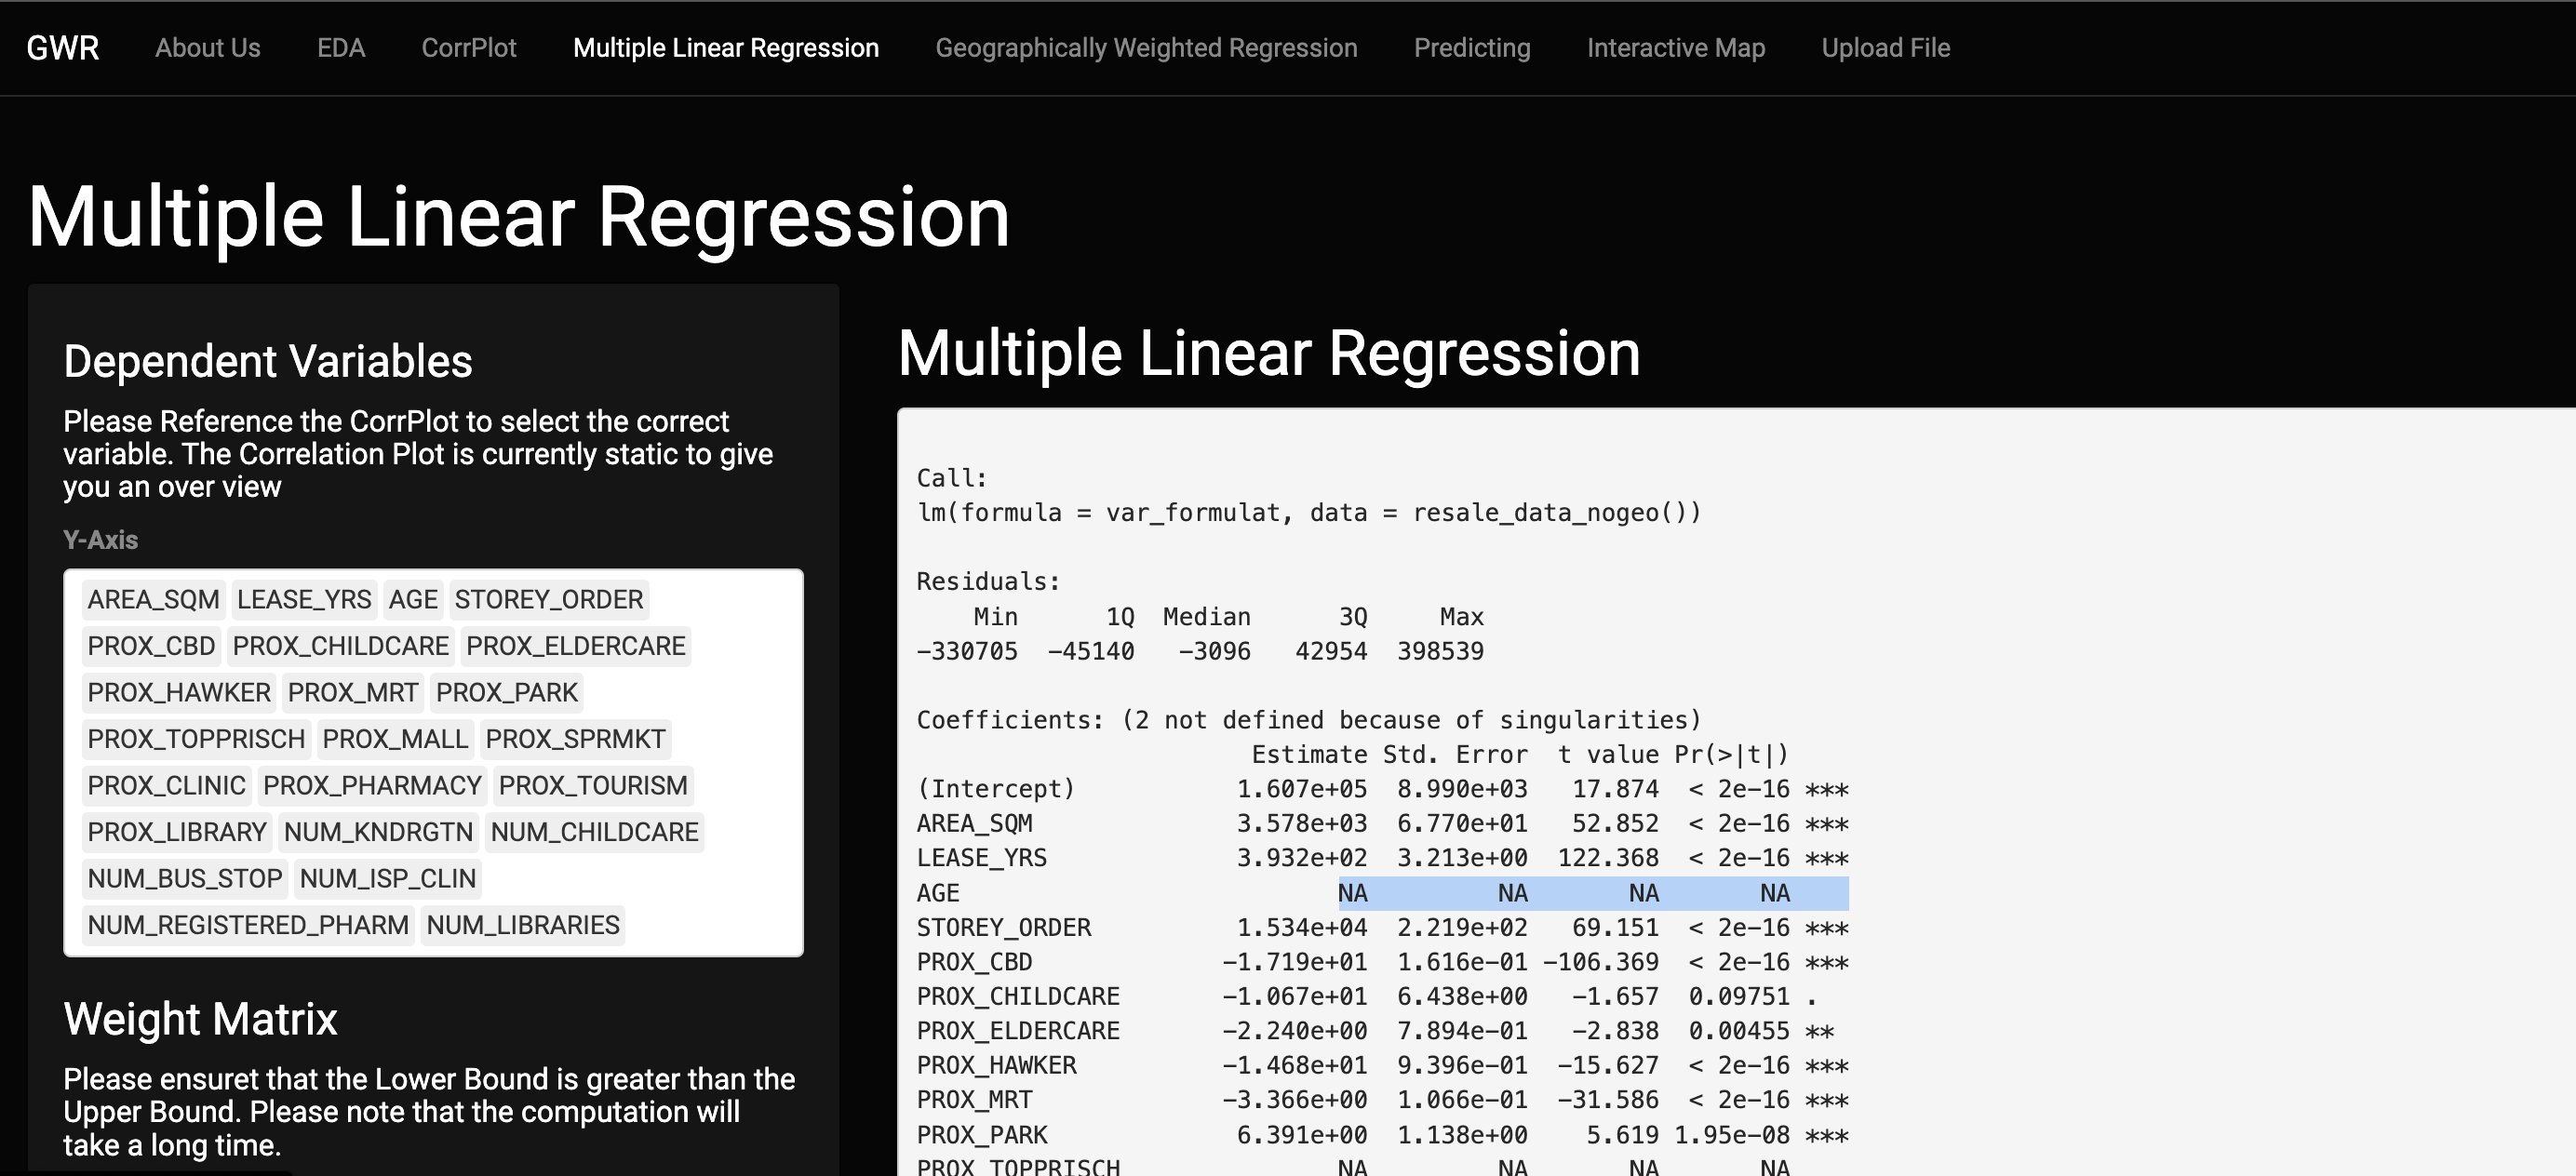
\includegraphics{images/Screenshot 2023-04-14 at 11.42.39 PM.png}

}

\caption{\label{fig-4}MLR Tab}

\end{figure}

\begin{figure}

{\centering 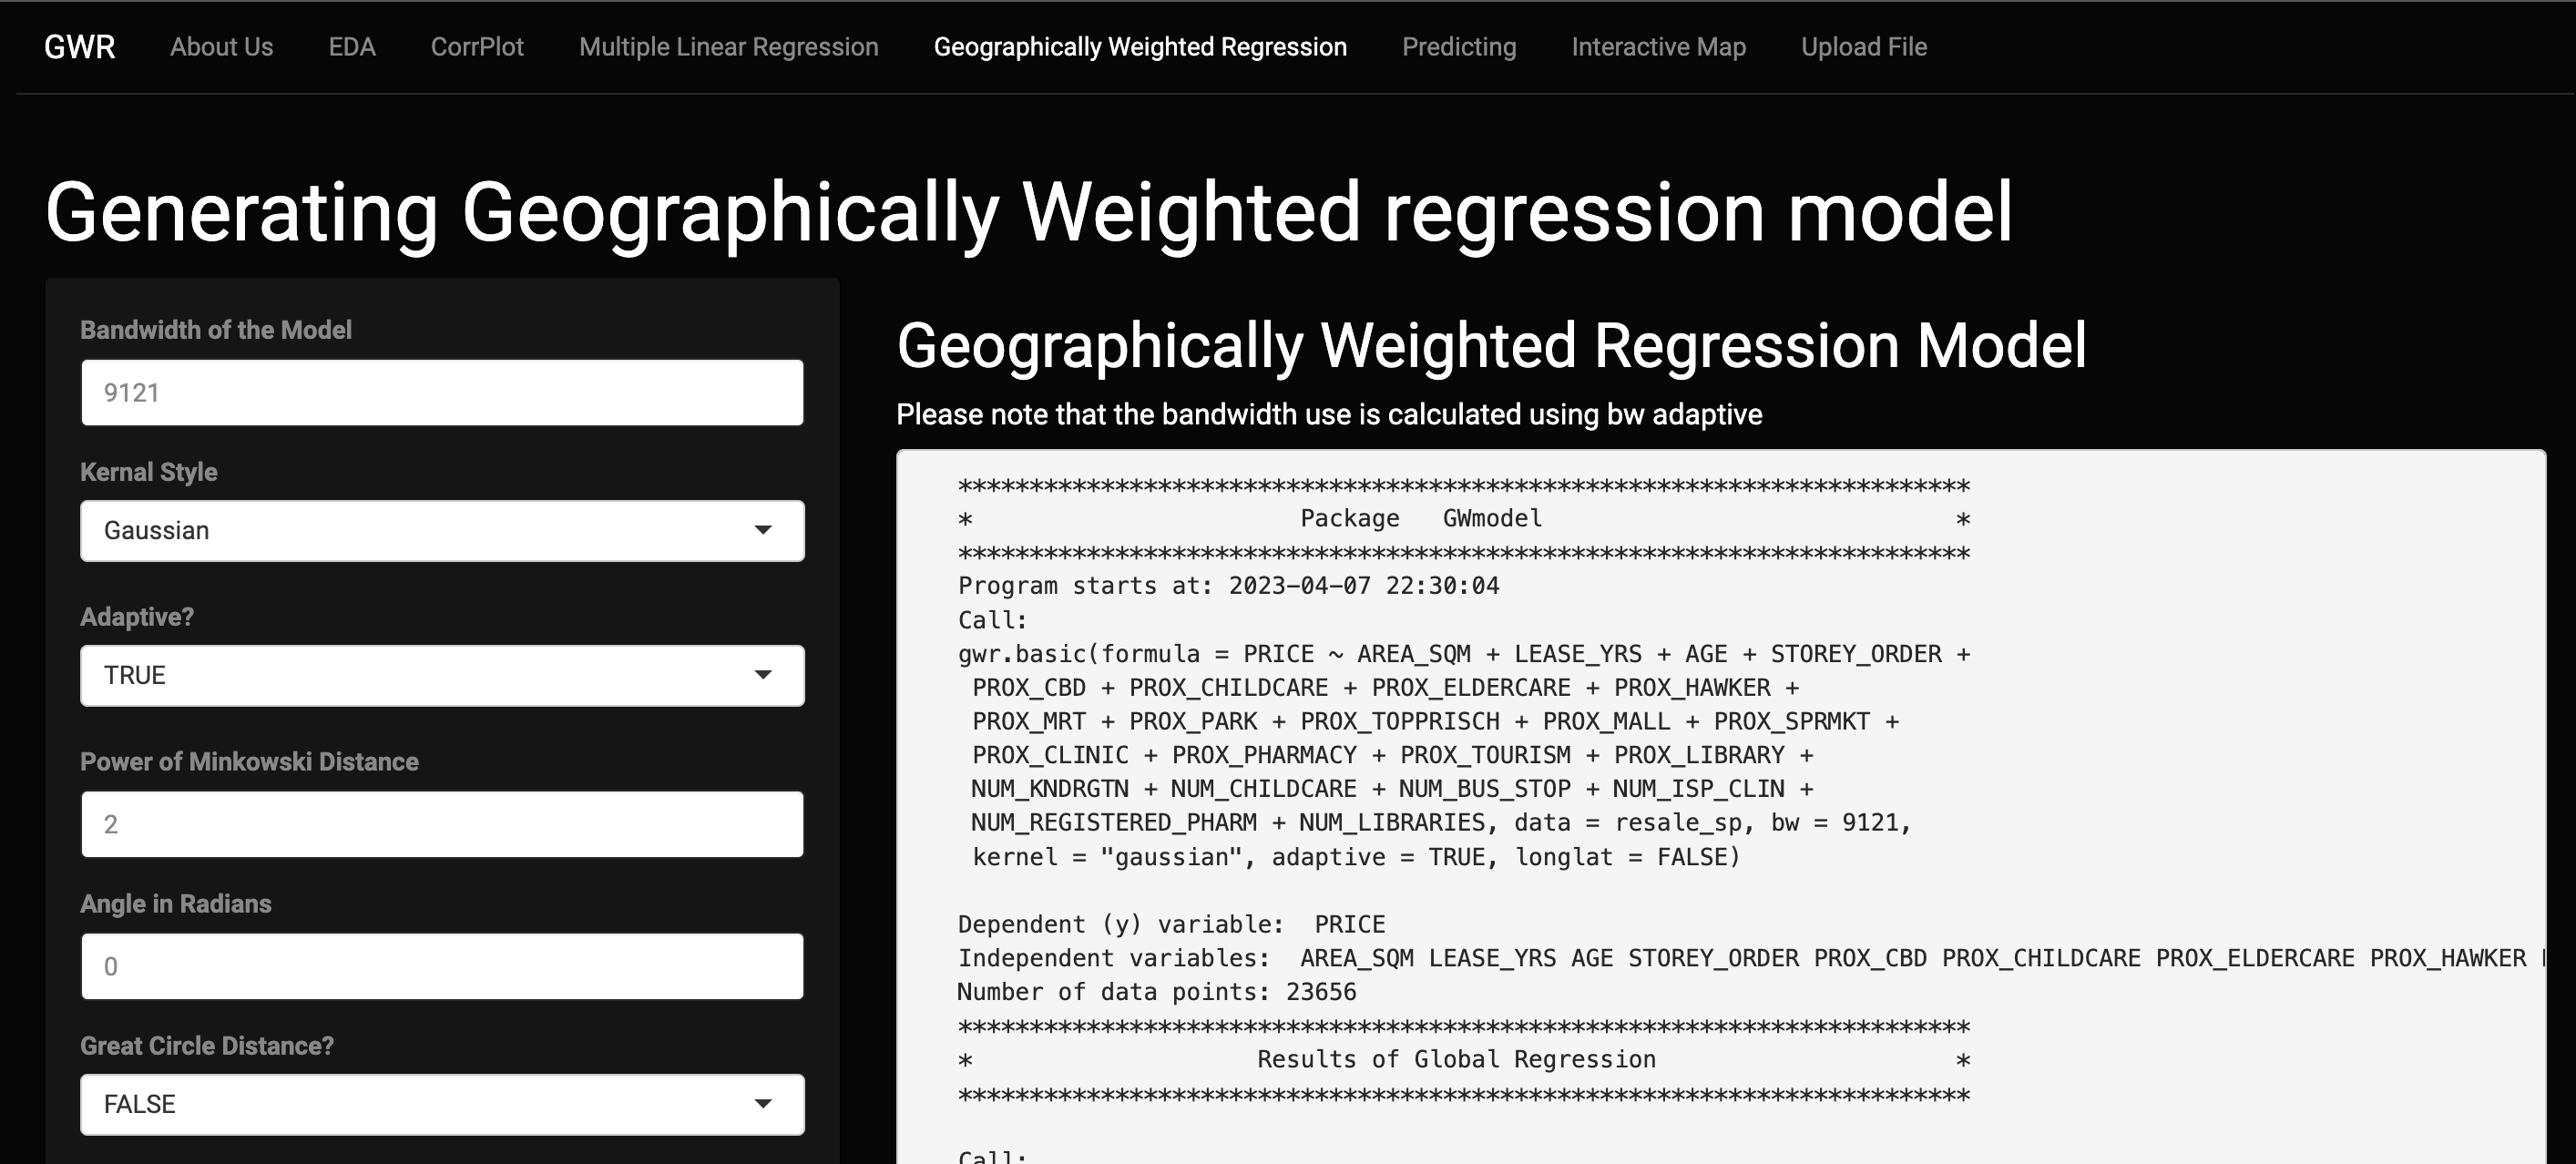
\includegraphics{images/Screenshot 2023-04-14 at 11.57.14 PM.png}

}

\caption{\label{fig-5}GWR Tab}

\end{figure}

\begin{figure}

{\centering 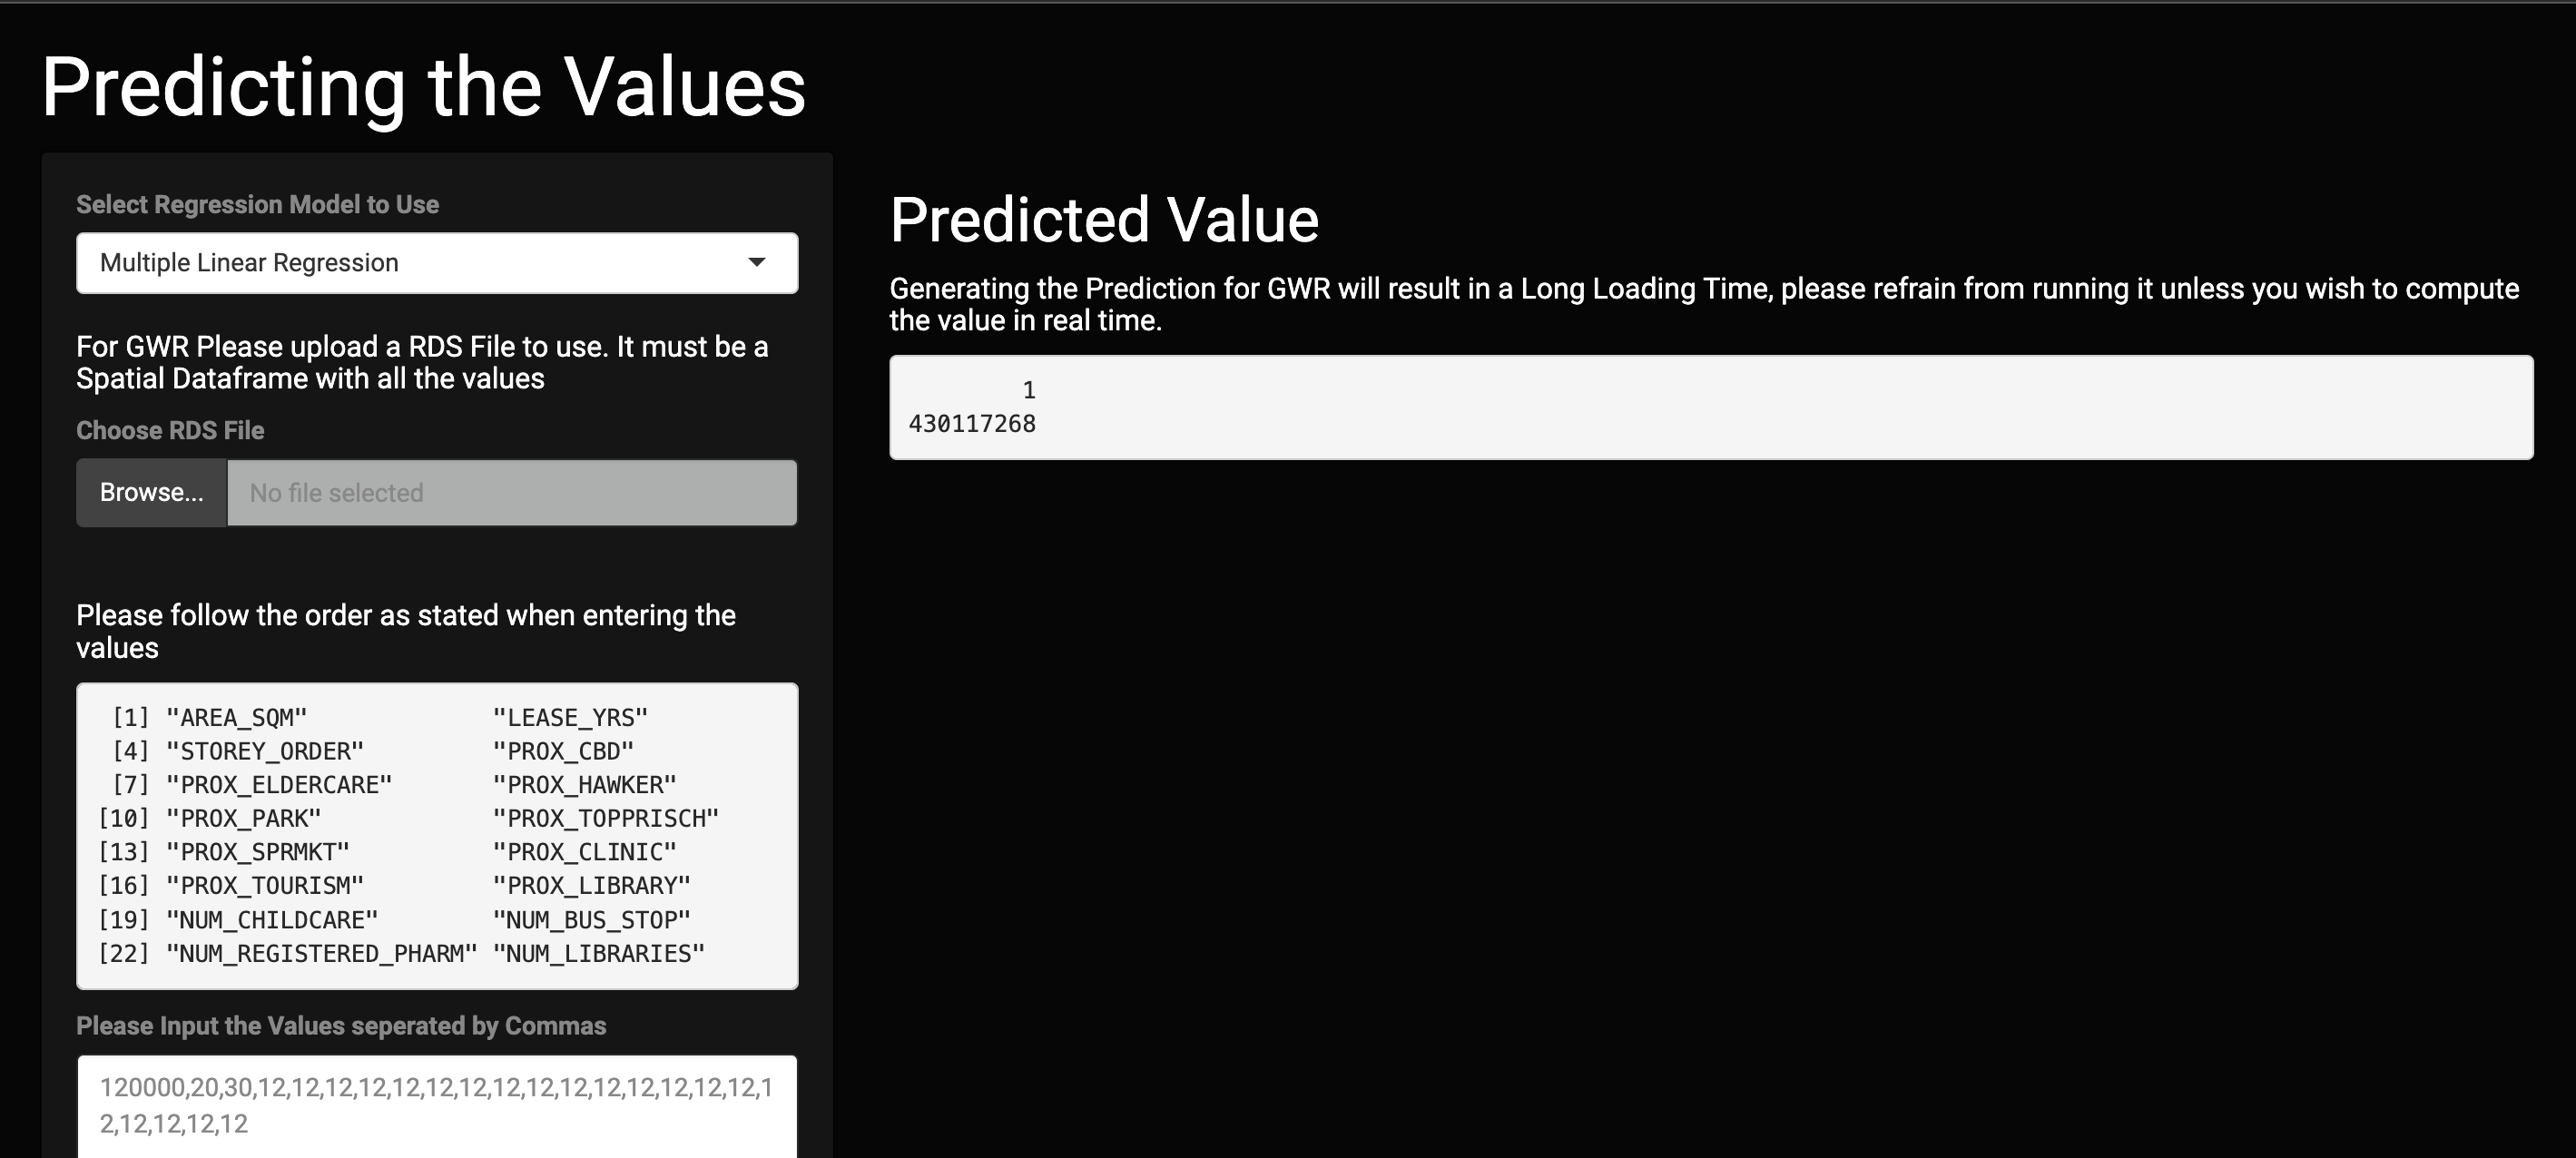
\includegraphics{images/Screenshot 2023-04-15 at 12.01.01 AM.png}

}

\caption{\label{fig-6}Predicting Tab}

\end{figure}

\begin{figure}

{\centering 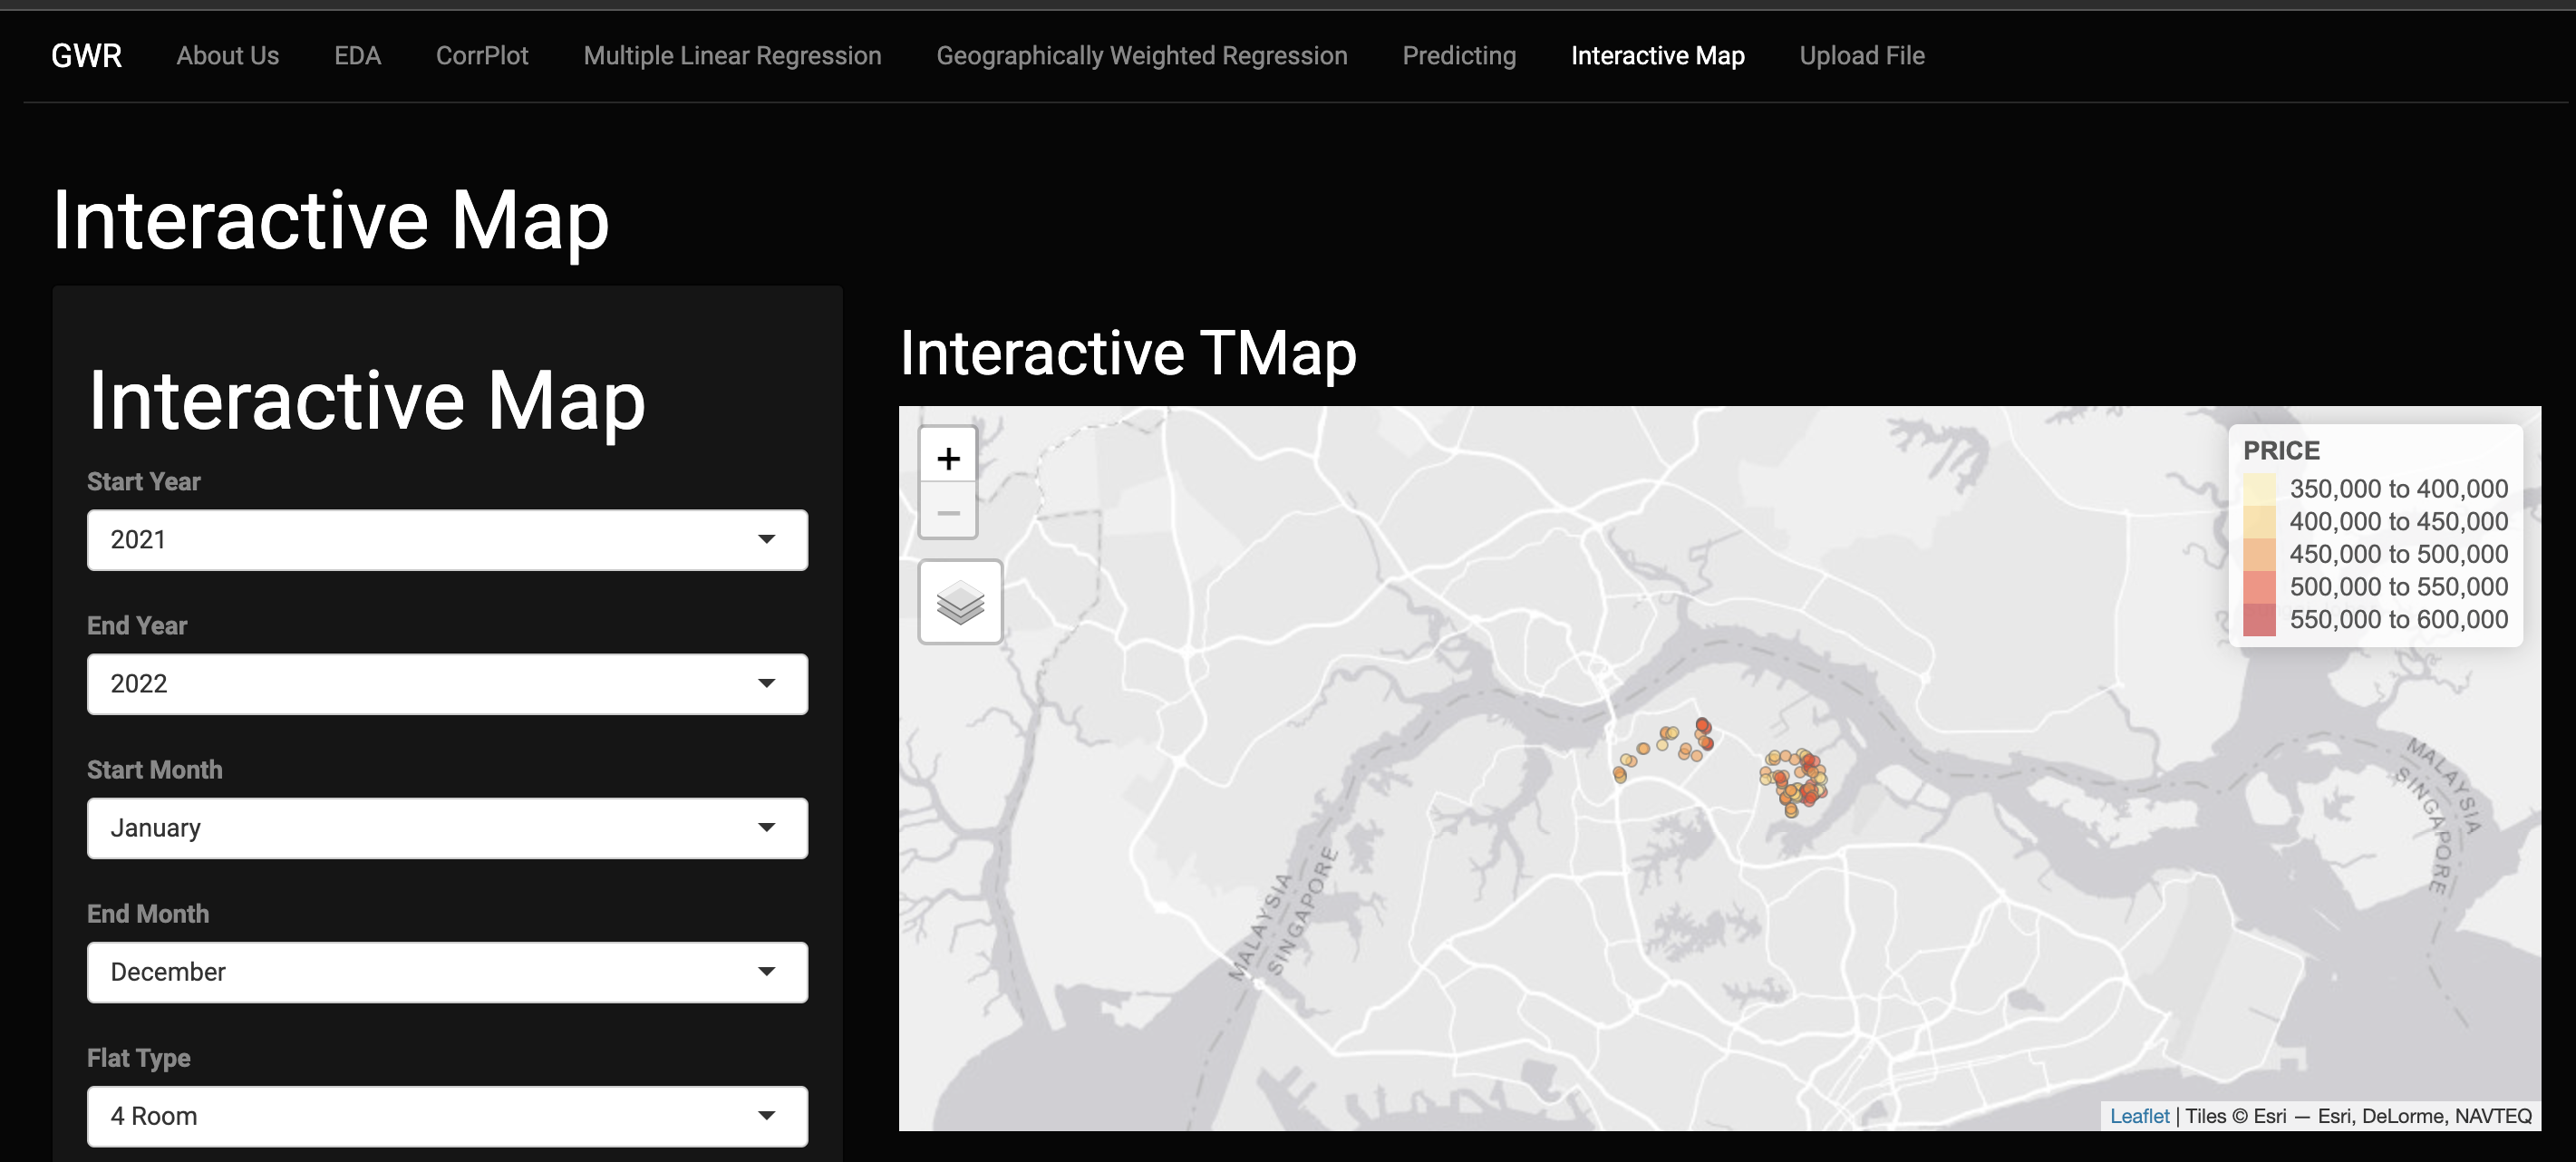
\includegraphics{images/Screenshot 2023-04-15 at 12.06.50 AM.png}

}

\caption{\label{fig-7}Interactive Map}

\end{figure}

\begin{figure}

{\centering 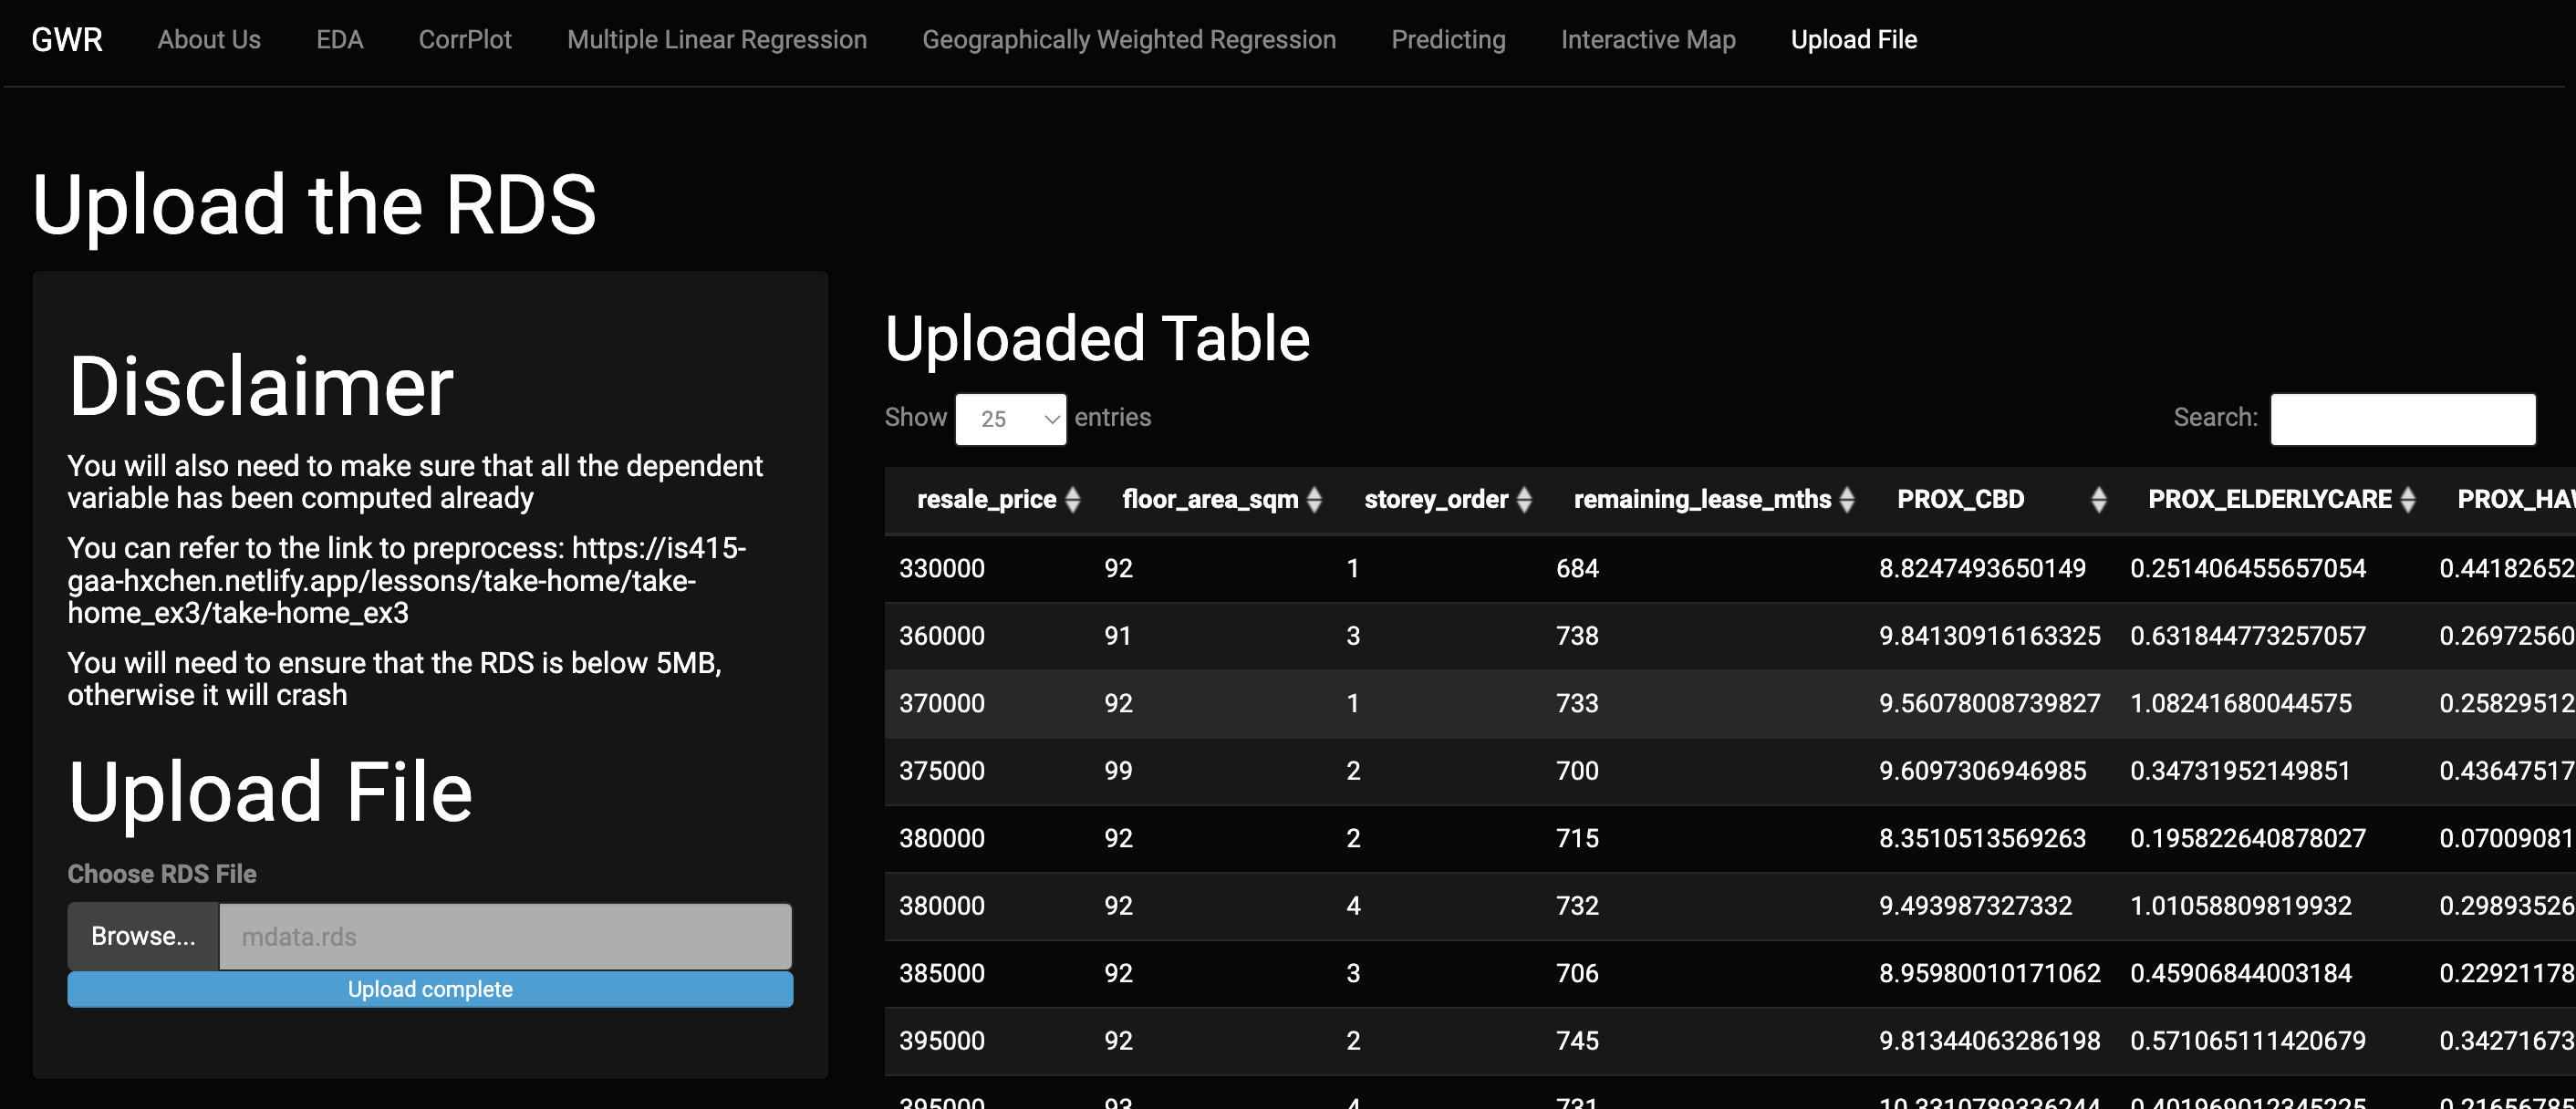
\includegraphics{images/Screenshot 2023-04-14 at 11.20.47 PM.png}

}

\caption{\label{fig-8}Upload Tab}

\end{figure}

\begin{figure}

{\centering 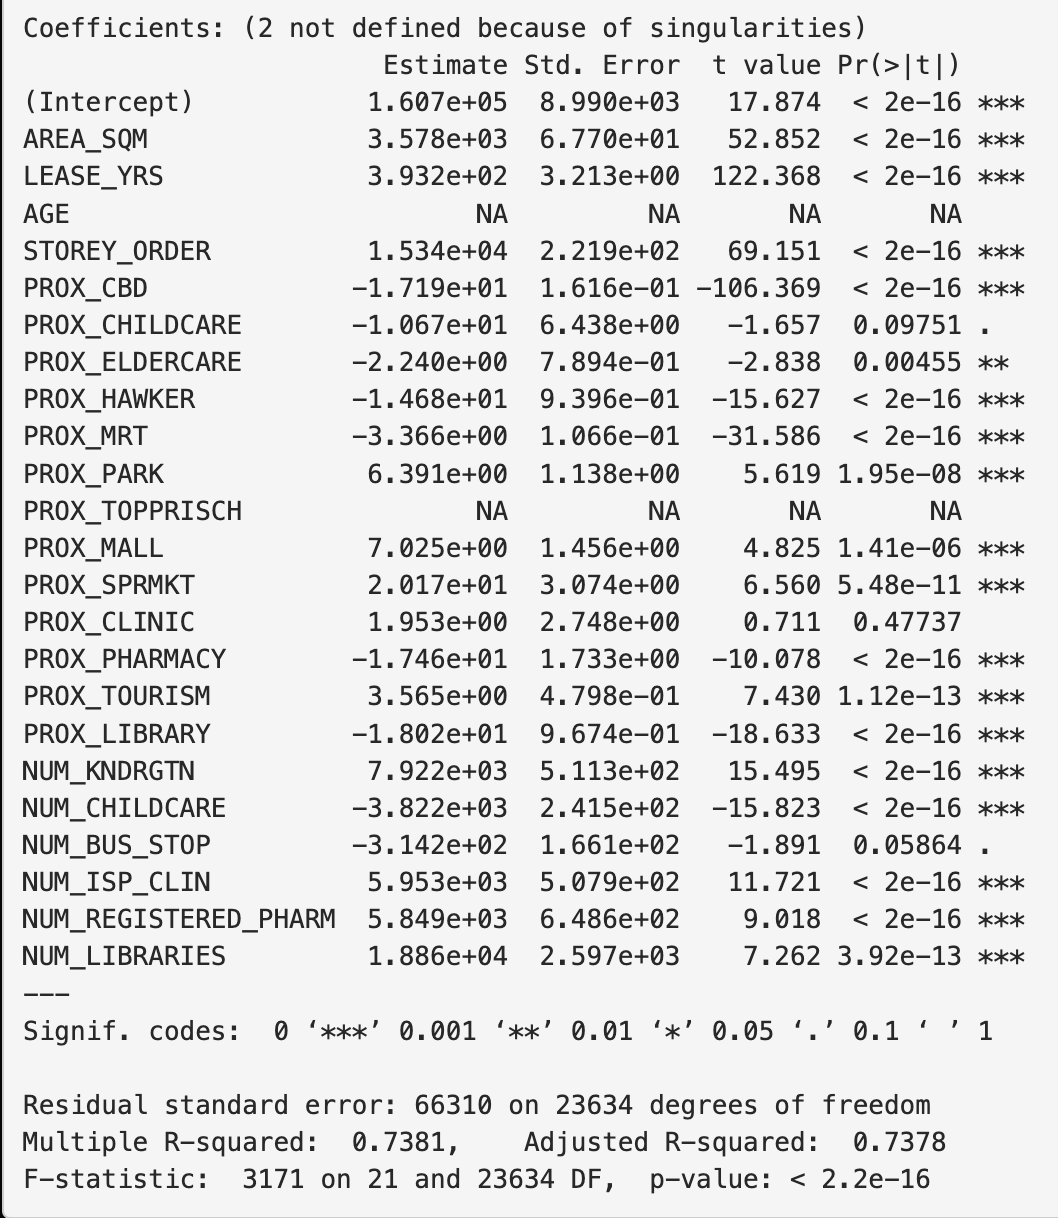
\includegraphics{images/Screenshot 2023-04-15 at 10.52.59 PM.png}

}

\caption{\label{fig-9}Linear Regression Score}

\end{figure}

\begin{figure}

{\centering 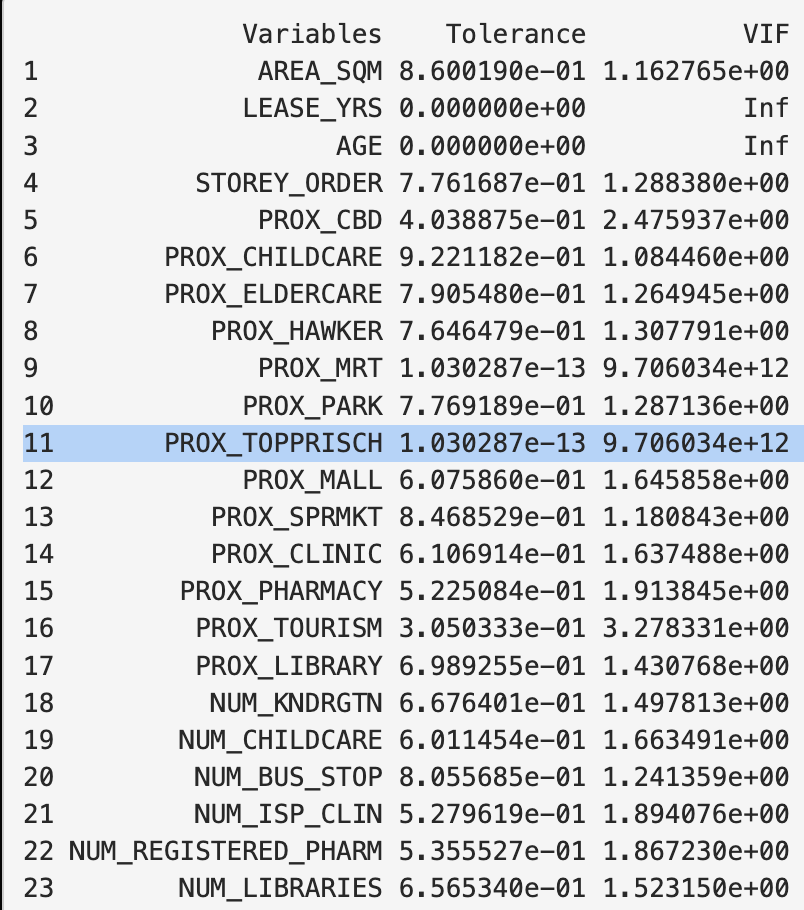
\includegraphics{images/Screenshot 2023-04-15 at 11.02.35 PM.png}

}

\caption{\label{fig-10}Linearity Test}

\end{figure}

\begin{figure}

{\centering 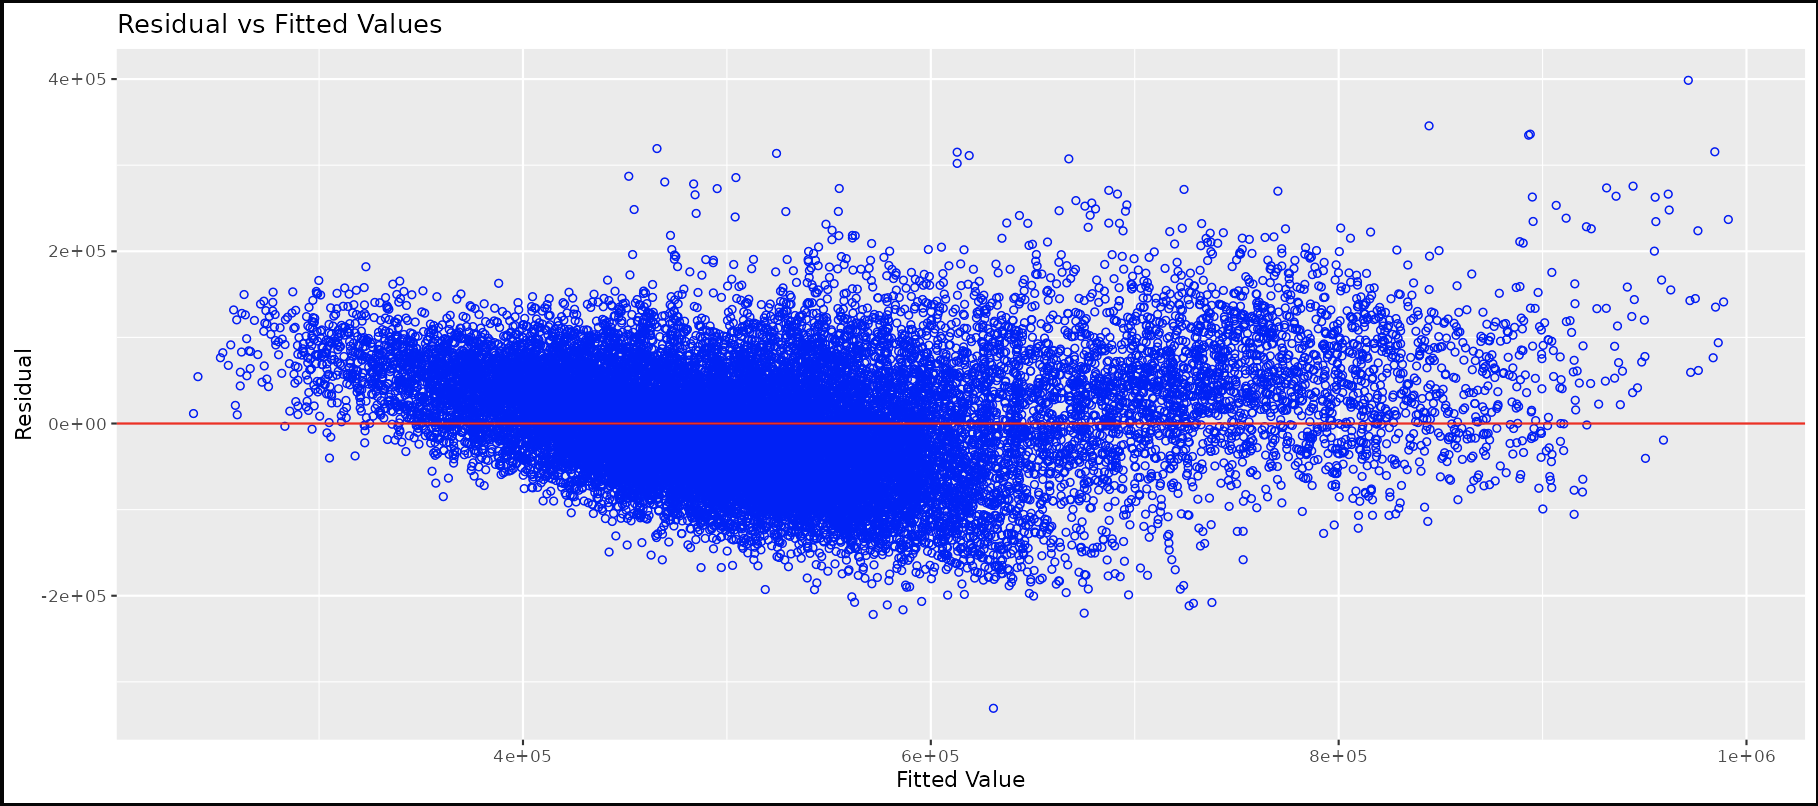
\includegraphics{images/Screenshot 2023-04-15 at 11.02.44 PM.png}

}

\caption{\label{fig-11}Homoscedasticity (Non Linearity)}

\end{figure}

\begin{figure}

{\centering 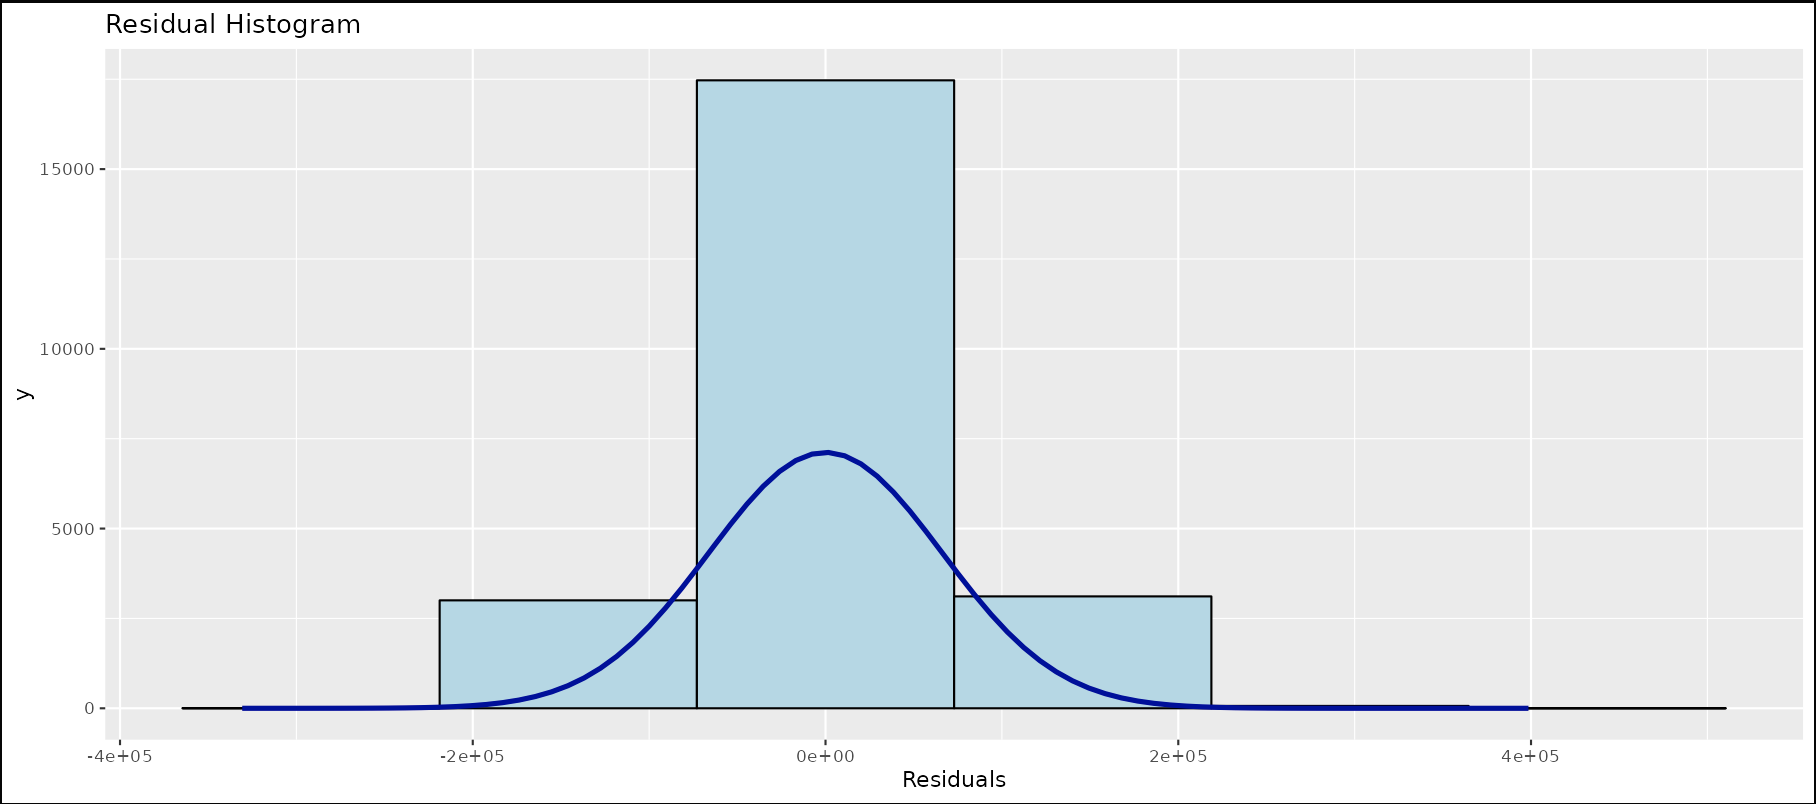
\includegraphics{images/Screenshot 2023-04-15 at 11.02.51 PM.png}

}

\caption{\label{fig-12}Normal Distribution of LM Model}

\end{figure}

\begin{figure}

{\centering 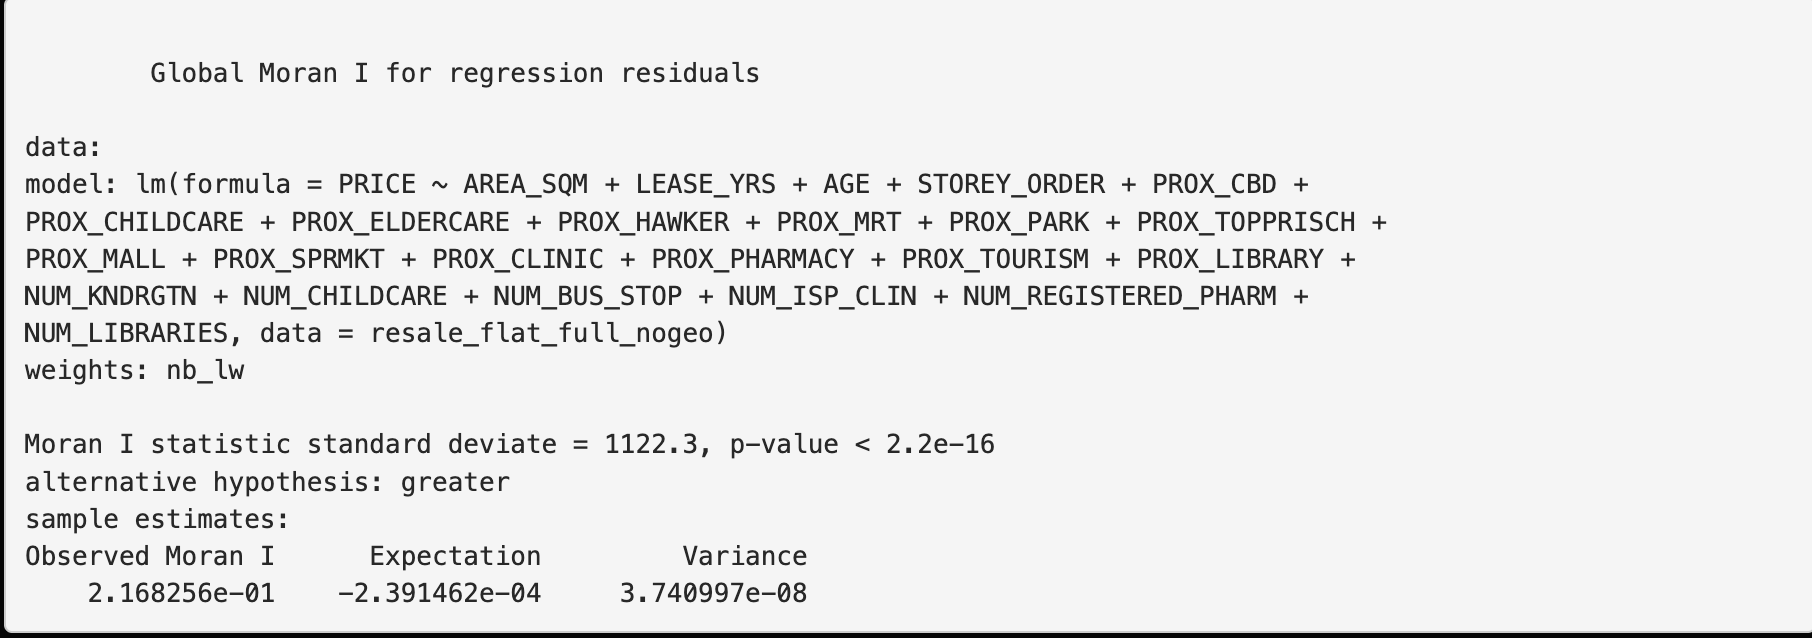
\includegraphics{images/Screenshot 2023-04-15 at 11.00.00 PM-01.png}

}

\caption{\label{fig-13}Moran I Test}

\end{figure}

\begin{figure}

{\centering 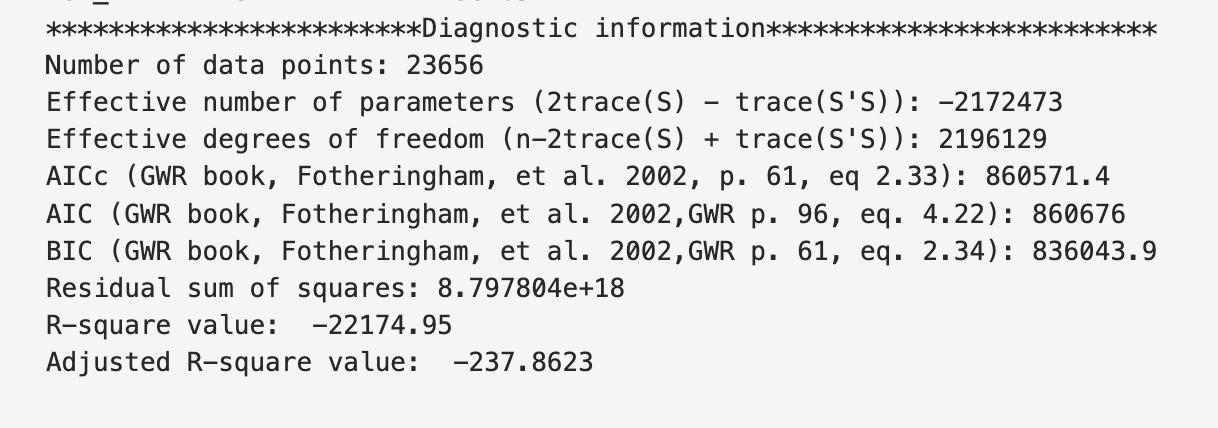
\includegraphics{images/Screenshot 2023-04-15 at 11.27.38 PM.png}

}

\caption{\label{fig-14}GWModel}

\end{figure}

%% begin pandoc before-bib
%% end pandoc before-bib
%% begin pandoc biblio
%% end pandoc biblio
%% begin pandoc include-after
%% end pandoc include-after
%% begin pandoc after-body
%% end pandoc after-body

\end{document}
\endinput
%%
%% End of file `sample-manuscript.tex'.
